{
\chapter{Background}
\color{black}

\section{Synchrotron-based X-ray tomographic microscopy}
\label{introduction:synchrotron-based-x-ray-microtomography}
X-ray radiography, discovered by R\"{o}ntgen in 1895 \cite{Roentgen1895}, is a 2D non-destructive imaging technique, that has played
a crucial role in various fields like medicine, material science, archeology, quality control and homeland security until these days. 
In the 1960s,
Cormack had the intuition that the density distribution of an object could be retrieved from radiographic projections
acquired around a single rotation axis \cite{Cormack1963} and
in the 1970s Hounsfield devised the first X-ray tomographic scanner \cite{Hounsfield1973}, upgrading radiography to 3D and 
giving birth to \emph{computed tomography (CT)}. CT scans have since been extensively utilized for preventive medicine and disease screening
\cite{Hsieh2009}. This method was later adopted for non-destructive testing in material research starting from the 1980s \cite{Reimers1983,Kanamori1986}.
In the same years, X-ray transmission tomography at micrometer scale was studied with synchrotron radiation \cite{Grodzins1983} and microfocus 
X-ray tubes \cite{Flannery1987}. 
\newline
Compared to laboratory sources, the major assets of X-rays produced at third-generation synchrotron facilities are:
the possibility of working with monochromatic light, therefore miminizing beam hardening effects; a few orders of magnitude higher flux, allowing 
much faster scans even with monochromatic light; an almost exact parallel beam geometry, which greatly simplifies tomographic reconstruction; 
partial transverse coherence of the X-ray beam enabling the usage of phase-contrast techniques. For all these reasons, 
reconstructions of synchrotron radiation based X-ray tomographic microscopy (SRXTM) data are affected by fewer artifacts and
feature a substantially improved contrast-to-noise-ratio (CNR) \cite{Bonse1996}.
\newline
In the last 20 years, SRXTM has found broad application in biology \cite{Ruegsegger1996,Westneat2003,Plouraboue2004,Cloetens2006,Betz2007,Lovric2013}, material science 
\cite{Baruchel2006,Beckmann2004,Uesugi2004,Lee1997,Wang2001,Snigirev1995,Cloetens1999} and paleontology \cite{Chen2006,Donoghue2006}.
\newline
The experimental data used for the studies conducted in this thesis were acquired at the TOMCAT beamline of
the Swiss Light Source (SLS) at the Paul Scherrer Institute (PSI), in operation since June 2006 \cite{Stampanoni2007}. 
X-rays are produced by a 2.9 T superbending magnet with a critical energy of 11.1 keV on a 2.4 GeV storage ring \cite{SLS2016}.
%and energies range from 6 up to 45 keV \cite{Stampanoni2007}.
A fixed-exit double crystal multilayer monochromator (DCMM)
located in the front-end allows to work with monochromatic light  in the 6 to 45 keV energy range \cite{Stampanoni2002}. X-rays exiting the sample are,
first, converted into visible light by a scintillator screen and,
then, projected onto a digital camera (CCD, CMOS or sCMOS) detector with suitable optics \cite{Lovric2013}. 
Thanks to interchangeable cameras, the field-of-view
(FOV) can range from 28.2$\times$ 23.8 mm$^{2}$ with 11 $\mu $m pixel size to
13.1$\times$ 13.1 mm$^{2}$ with 6.5 $\mu $m pixel size. Objectives placed between the scintillator screen and the camera can 
yield an up to 40-fold magnification of the FOV, allowing to reach an effective pixel size down to 0.16 $\mu $m.

\section{X-ray projections}
\subsection{Beer-Lambert law}
\label{introduction:beer-lambert-law}
X-ray photons traveling through a material either interact with particles of mass or pass unaffected. Interactions occur every time
a photon is absorbed, due to the photoelectric effect, or is scattered, due to the Compton (incoherent scattering) or 
Rayleigh (coherent scattering) effect. 
In all these scenarios, photons are considered removed from the original beam.  The loss of photons caused by absorption and scattering is called \emph{attenuation}.
\newline
Assuming that $N_{\text{in}}$ X-ray photons move in parallel geometry along the $z$-axis and
hit perpendicularly an infinitesimally thin (thickness $\Delta z \approx 0$) and homogeneous slab of material, 
the Beer-Lambert law states that the expected number of photons lost inside the body is directly proportional to $N_{\text{in}}$ and $\Delta z$
\cite{Bouger1729,Lambert1760,Beer1852}:
\begin{equation}
  \Delta N := N_{\text{out}} - N_{\text{in}} = -\mu N_{\text{in}}\Delta z \hspace{0.3cm},
  \label{beer_lambert_law_1}
\end{equation}
where $\mu$ is called \emph{linear attenuation coefficient}, has units of an inverse length and represents 
a characteristic quantity of a given material. It holds that:
\begin{equation}
  \frac{\mu}{\rho} = \frac{\sigma_{\text{tot}}}{uA} \hspace{0.5cm},
\end{equation}
where $\rho$ is the density, $u$ is the atomic mass unit, $A$ is the relative atomic mass and $\sigma_{\text{tot}}$
is the total cross section, accounting for all types of interactions between X-rays and the selected material.
Considering the differential form 
of (\ref{beer_lambert_law_1}) and integrating over the thickness of the slab $l$, the Beer-Lambert law becomes:
\begin{equation}
  N_{\text{out}} = N_{\text{in}}\:\exp\left(-\mu l\right) \hspace{0.3cm}.
   \label{beer_lambert_law_2} 
\end{equation}
If the body consists of $n_{s}$ thin slabs with different materials whose thicknesses $z_{i}$
sum up to $l$, (\ref{beer_lambert_law_2}) assumes a more general form:
\begin{equation}
  N_{\text{out}} = N_{\text{in}}\:\exp\left( -\sum\limits_{i=0}^{n_{s}}\mu_{i}z_{i} \right)\Bigg|_{\sum\limits_{i=0}^{n_{s}}z_{i} = l}
                 \overset{\mathclap{\substack{z_{i} \longrightarrow 0\,\,,\,\forall\:i\\[2pt]n_{s} \longrightarrow \infty}}}{=}
                 \hspace{0.6cm}N_{\text{in}}\:\exp\left({-\int\limits_{0}^{l}\mu(z)dz}\right) \hspace{0.3cm}.
   \label{beer_lambert_law_3} 
\end{equation}
Since, in practice, the X-ray source provides a flux of photons, it is convenient to rewrite (\ref{beer_lambert_law_3}) in terms of 
\emph{intensities}, defined in general as the number of photons impinging on a selected region per unit of time:
\begin{equation}
  I_{\text{out}} = I_{\text{in}}\:\exp\left( -\sum\limits_{i=0}^{n_{s}}\mu_{i}z_{i} \right)\Bigg|_{\sum\limits_{i=0}^{n_{s}}z_{i} = l}
                 \overset{\mathclap{\substack{z_{i} \longrightarrow 0\,\,,\,\forall\:i\\[2pt]n_{s} \longrightarrow \infty}}}{=}
                 \hspace{0.6cm}I_{\text{in}}\:\exp\left(-\int\limits_{0}^{l}\mu(z)dz\right) \hspace{0.3cm}.
   \label{beer_lambert_law_4} 
\end{equation}
$I_{\text{out}}$ is called \emph{projection image} of $\mu$. Relation (\ref{beer_lambert_law_4}) is valid only under the following conditions:
%\begin{itemize}
 %\setlength\itemsep{0.1em} 
 %\item 
 (i) interactions act independently from each other;
 %\item the attenuating medium must not scatter the radiation;
 %\item
 (ii) the incident radiation consists of parallel rays;
 %\item
 (iii) the X-ray beam is monochromatic, otherwise (\ref{beer_lambert_law_4}) has to be rewritten for each single energy component $\Energy$
       by replacing $I_{\text{out}}$, $I_{\text{in}}$ and $\mu(z)$ with $I_{\text{out}}\left(\Energy\right)$, $I_{\text{in}}\left(\Energy\right)$
       and $\mu\left(z,\Energy\right)$.
%\end{itemize}
\newline
At SLS, X-rays are shaped to have a divergence angle between 0.6 mrad and 2 mrad \cite{SLS2016}, allowing
the parallel beam geometry to be a good approximation. The DCMM provides monochromatic radiation with $\Delta\lambda/\lambda$
($\lambda$ is the wavelength) of a few percent when multilayer crystals are used or $10^{-4}$ when the Si-111 crystals are used \cite{SLSOptics2016}.
\newline
Despite its simplicity, the Beer-Lambert law is the physical principle
%ruling the mechanism of \emph{X-ray absorption imaging},
%which corresponds to standard radiography
providing the basis for the mathematical model of tomographic reconstruction.

\subsection{Absorption-contrast imaging}
Standard \emph{X-ray absorption imaging} can be performed on materials and at energies where $\mu = \mu_{a} + \mu_{s} \approx \mu_{a}$, 
$\mu_{a}$ being the absorption coefficient and $\mu_{s}$ the scattering coefficient.
The cross-section of the photoelectric effect, ruling the absorption of X-ray photons inside the sample, is $\propto Z^{3}/E^{3}$ \cite{WikiPhoto},
where $Z$ is the atomic number and $E$ the beam energy.
X-ray absorption imaging can well discriminate between hard and soft tissues, as $\mu_{a}$ varies considerably
for materials with so disparate densities. On the other hand, it fails to provide enough contrast between different types
of soft tissues due to the little variation of $\mu_{a}$.

\subsection{Phase-contrast imaging}
\label{introduction:phase-contrast-imaging}
% X-ray absorption imaging can discriminate between hard and soft tissues, because the attenuation coefficient is a function of the
% material density: heavier elements like bones and teeth have a much higher absorption cross section and, therefore, bigger attenuation
% coefficient than lighter elements forming soft tissues. Standard radiography usually fails to provide enough contrast between different types
% of soft tissues, as the range of attenuation coefficients results very small.
% \newline
At X-ray energies, the refractive index $n$ of a material is expressed as follows \cite{Nielsen2011}:
\begin{align}
  n &= 1 - \delta + i\beta \label{introduction:refractive-index}\\[0.5em]
  \text{where}\hspace*{1.0cm}\beta &= \frac{\mu_{a}\lambda}{4\pi} \label{introduction:beta}\\[0.5em]
  \text{and}\hspace*{1.0cm}\delta &= \frac{\lambda^{2}r_{e}n_{e}}{2\pi}\hspace*{0.5cm}, \label{introduction:delta} 
\end{align}
where $r_{e}$ is the classical radius of the electron and $n_{e}$ the electron density of the material. 
The terms $\beta$ and $\delta$ are related to different interactions between X-rays and the sample: $\beta$ accounts for the absorption, which affects the amplitude of the X-ray wave front \cite{Veen2004};
$\delta$ accounts for the coherent Rayleigh scattering \cite{Nielsen2011}, which affects the phase of the X-ray front wave \cite{Veen2004}.
\newline
\textit{Phase-contrast} is an imaging modality sensitive to variations of $\delta$, thus, of electron density according to (\ref{introduction:delta}).
Soft tissues can be effectively discriminated when $\lambda < 0.1$ nm and
phase-contrast dominates absorption contrast \cite{Nielsen2011,Veen2004}.
% Thus, contrast is provided by differences in electron densities rather than differences in material densities.
Phase-contrast techniques measure phase variations of a spatially coeherent X-ray beam.
% , that can be easily produced by third generation synchrotrons.
Since it is not possible to fabricate detectors with response time comparable to the oscillation of optical or quantum fields,
the phase of the wave front cannot be measured directly \cite{Modregger2012}.
There are various systems to convert X-ray phase variations into
intensity variations measurable at the detector. Examples are propagation-based phase contrast \cite{Snigirev1995,Wilkins1996}, 
differential phase contrast based on a Talbot grating interferometer \cite{David2002}, analyzer-based phase contrast \cite{Davis1995} and crystal-based interferometry \cite{Momose1996}.
\newline
In this work, we addressed the reconstruction of projections created by propagation-based and differential phase contrast.


\subsubsection{Propagation-based phase-contrast projections}
\label{introduction:phase-contrast-imaging:propagation-based-phase-contrast-projections}
Propagation-based phase-contrast (PBPC) (also called ``in-line phase-contrast'') is yielded by the free-space propagation
of the X-ray wave front coherently scattered by the sample \cite{Snigirev1995,Wilkins1996} and is based on the Fresnel approximation of the Kirchoff diffraction formula
\cite{Goodman2005}. For absorption contrast imaging,
the detector is located directly behind the object.
The opposite is true for PBPC, where a certain distance is necessary to obtain edge enhancement.
\newline
 Methods based on the \emph{contrast-transfer function (CTF)} \cite{Guigay1977} and the \emph{transport of intensity equation (TIE)} 
 \cite{Teague1983,Rytov2011} offer a way to retrieve the phase from the intensity data. CTF works under the condition that the sample is 
 weakly absorbing \cite{Langer2008}; it also requires high coherence and the acquisition of 
 projections at multiple distances \cite{Cloetens1999}. TIE is a preferable
 solution when the beam coeherence is limited \cite{Paganin2002}. 
\newline 
The phase of the PBPC projections used in this work are retrieved by the Paganin algorithm \cite{Paganin2002},
that inverts the TIE equation and is applicable under the following assumptions: (i) ``near-field'' condition, i.e. short detector-sample distance;
 (ii) the \emph{projection} and \emph{paraxial} approximations are valid \cite{Paganin2006}; (iii) the sample consists of a single material.
% The projection approximation assumes that the scatterers are very weak and minimally deviate photons from
% their original path; in this way, phase and amplitude of the X-ray beam at the exit surface of the sample can be considered a function
% of phase and amplitude shifts accumulated along each ray path \cite{Paganin2006}. As a result,
% a \emph{phase projection} is considered a collection of line integrals through the phase map characterizing the object under study.
% \newline
% The paraxial approximation states that rays form only small angles with the propagation axis. 
% \newline
% The propagation of a monochromatic scalar wave field with angular frequency $\omega$, $\psi(x,y,z)\:\exp\left(-i\omega t\right)$ 
% ($i$ is the imaginary unit), in an uncharged,
% non-conducting and non-magnetic medium is ruled by the Helmholtz equation \cite{Born1999}:
% \begin{equation}
%   \left[ \nabla^{2} + n(x,y,z)\:k^{2} \right]\:\psi(x,y,z) = 0 \hspace{0.3cm},
%   \label{paganin_1}
% \end{equation}
% where $\nabla^{2}$ is the Laplacian operator, $k = 2\pi/\lambda$ and $\lambda$ is the wavelength.
% $n(x,y,z)$ is the refractive index, expressed for X-rays in the form $n = 1-\delta + i\beta$ with $\delta,\,\beta \in \mathbb{R}_{0}^{+}$,
% since usually $n \approx 1$. $\delta$ is proportional to the electron density, whereas $\beta$ to the linear attenuation coefficient $\mu$.
% If the wave field propagates along $z$ under the paraxial approximation, (\ref{paganin_1}) simplifies to \cite{Paganin2006}:
% \begin{equation}
%   \left( 2ik\frac{\partial}{\partial z} + \nabla_{\bot}^{2}\right) \psi(x,y,z) = 0 \hspace{0.3cm},
%     \label{paganin_2}
% \end{equation}
% where $\nabla_{\bot}^{2} = \partial^{2}/\partial^{2}x + \partial^{2}/\partial^{2}y$ is the Laplacian operator in the transverse plane.
% By rewriting the wave field in terms of its intensity $I(x,y,z) = |\psi(x,y,z)|^{2}$ and phase $\phi(x,y,z) = \arg\:\psi(x,y,z)$ as
% $\psi(x,y,z) = \sqrt{I(x,y,z)}\exp(i\phi(x,y,z))$, TIE is obtained \cite{Teague1983,Rytov2011}:
% \begin{equation}
%   -k\:\frac{\partial}{\partial z}I(x,y,z) = \nabla_{\bot} \cdot \left( I(x,y,z)\:\nabla_{\bot}\phi(x,y,z) \right) \hspace{0.3cm}.
%     \label{paganin_3}
% \end{equation}
% Paganin algorithm is based on the assumption that the object under study is composed of a single material.
% The wave field intensity at the exit surface, $z=0$, can, therefore, be approximated by the Beer-lambert law as \cite{Paganin2002}:
% \begin{equation}
%   I(x,y,z=0) = I_{\text{in}}\:\exp\left(-\mu l(x,y)\right) \hspace{0.3cm},
%     \label{paganin_4}
% \end{equation}
% where $I_{\text{in}}$ and $\mu$ have already been introduced in \ref{introduction:beer-lambert-law} and
% $l(x,y)$ is the object thickness projected onto the plane $z=0$. For a sufficiently thin object, the phase $\phi(x,y,z=0)$ is
% proportional to $l(x,y)$:
% \begin{equation}
%   \phi(x,y,z=0) = -\frac{2\pi}{\lambda}\delta\:l(x,y) \hspace{0.3cm}.
%    \label{paganin_5}
% \end{equation}
% Moreover, assuming a very small propagation distance $dz$ between the exit surface and the detector plane
% and using (\ref{paganin_4}), the left side of
% (\ref{paganin_3}) simplifies into:
% \begin{equation}
%   \frac{\partial}{\partial z}I(x,y,z=0) \approx \frac{I(x,y,z=dz) - I_{\text{in}}\:\exp\left(-\mu l(x,y)\right)}{dz}\hspace{0.3cm}.
%    \label{paganin_6}
% \end{equation}
% By substituting (\ref{beer_lambert_law_4}) and (\ref{paganin_6}) into (\ref{paganin_3}), one obtains \cite{Paganin2002}:
% \begin{equation}
%   \left(-\frac{dz \cdot \delta}{\mu}\nabla_{\bot}^{2} + 1\right)\exp\left(-\mu l(x,y)\right) = \frac{I(x,y,z=dz)}{I_{\text{in}}} \hspace{0.3cm}.
%   \label{paganin_7}
% \end{equation}
% Equation (\ref{paganin_7}) can be easily inverted with respect to $l(x,y)$; thanks to (\ref{paganin_5}), $\phi(x,y,z=0)$
% can be computed by means of the Fourier Transform $\Four$ \cite{Paganin2002}:
Calling $k_{x}$ and $k_{y}$ the dual Fourier variables of $x$ and $y$,
$I(x,y,z=\delta z)$ the intensity measured at distance $\delta z$ from the sample, the projected phase $\phi$ is retrieved by the Paganin algorithm
as \cite{Paganin2002}:
\begin{equation}
  \phi(x,y,z=0) = \frac{2\pi}{\lambda}\frac{\delta}{\mu} \ln\left( \Four_{x,y}^{-1}\left\{ \mu 
                  \frac{\displaystyle\Four_{x,y}\left\{\frac{I(x,y,z=dz)}{I_{\text{in}}}\right\}}{dz\:\delta\sqrt{k_{x}^{2}+k_{y}^{2}} + \mu} \right\} \right) \hspace{0.3cm},
  \label{paganin_8}
\end{equation}
with
\begin{equation}
  \Four_{x,y}\left\{f(x,y)\right\} = \int\limits_{0}^{\infty}dx\int\limits_{0}^{\infty}dy \: f(x,y)\exp\left(i\left(k_{x}x + k_{y}y\right)\right) \hspace{0.3cm}.
  \label{paganin_9}
\end{equation}
being the Fourier transform.
Formula (\ref{paganin_8}) clearly shows that Paganin phase retrieval works as a low-pass filter on the input intensity data $I(x,y,z=dz)$,
since the kernel $1/\left(a_{1}\sqrt{k_{x}^{2}+k_{y}^{2}} + a_{2}\right)$ attenuates more frequency components corresponding to
high values of $k_{x}$ and $k_{y}$.
\newline
$\phi(x,y,z=0)$ represents the projected phase of the object. Once phase projections are acquired at different angular positions,
tomographic reconstruction techniques can provide the entire 3D phase map of the object. 
\newline
Compared to other methods, Paganin phase retrieval has the advantage of being fast and requiring single projections. Although quantitative results
are not achievable when the sample consists of two or more materials, Paganin can still be applied to enhance the contrast-to-noise ratio of the projections.


\subsubsection{Differential phase-contrast projections}
\label{introduction:phase-contrast-imaging:differential-phase-contrast-projections}
A \emph{grating interferometer (GI)} \cite{David2002,Momose2003} is a setup consisting of two gratings located after the source and the sample.
The first grating, G1 with period $p_{1}$, splits the incident beam into several diffraction orders, which interfere
constructively at specific distances if the beam features sufficient spatial coherence. 
The second grating, G2 with period $p_{2}$, is made of highly absorbing materials and is positioned in front of the detector
to analyze the interference pattern, whose period would be too small to be resolved otherwise.
\newline
GI is based on the occurrence of a rectangular-shaped interference pattern due to the \emph{Talbot effect} \cite{Talbot1836}.
Once the sample is placed inside the incident wave, the phase sensitivity of GI is given by the lateral shift of the interference pattern.
Assuming the gratings aligned along the $x$-axis (i.e. the line of the gratings are vertical), the lateral shift $\Delta x$ is proportional to the refraction angle $\alpha$, which, in turn, is proportional to the first derivative
of the phase of the wave of front after having traversed the sample \cite{Born1999,Modregger2012}:
\begin{equation}
  \alpha = -\frac{1}{k}\frac{\partial \phi}{\partial x} \hspace{0.3cm},
  \label{gi_dpc_1}
\end{equation}
where $k = 2\pi/\lambda$.
\newline
\emph{Phase-stepping} is a widely adopted procedure to analyze the signal at the detector:
one grating is shifted by fractions of its pitch with respect to the other grating and at each step a projection is acquired \cite{Modregger2012}.
The result is an oscillatory triangular function for each pixel, that looks closer to a sinusoid due to the finite spatial coherence of the system.
The phase stepping curve, $\varphi(\phi)$, is of the form \cite{Momose2006}:
\begin{equation}
    \varphi(\phi) = a_{1} + a_{2}\sin(\phi-p) \hspace{0.3cm},
\end{equation}
$a_{1}$, being the mean of $\varphi$, is connected to the absorption contrast;
$a_{2}$, being the amplitude of $\varphi$, is connected to the scatter contrast; 
$s$ is the lateral offset of the phase steps; $p$ is the phase of $\varphi$ and relates to the 
differential phase contrast (DPC). In particular, if $\varphi(\phi)_{1}$ and $\varphi(\phi)_{0}$ are
the phase stepping curves acquired with and without sample, DPC is given by \cite{Modregger2012}:
\begin{equation}
  \text{DPC} = \arg\Big(\Four\{\varphi(\phi)_{1}\}(q_{n})\Big) - \arg\Big(\Four\{\varphi(\phi)_{0}\}(q_{n})\Big) \hspace{0.3cm},
\end{equation}
where $q_{n}$ is the $n$-th Fourier harmonic and $n$ is the number of phase steps.
DPC is proportional to $\alpha$ according to \cite{Modregger2012}:
\begin{equation}
  \text{DPC} = 2\pi\frac{d_{m}\alpha}{p_{2}} \hspace{0.3cm},
   \label{gi_dpc_2} 
\end{equation}
where $d_{m}$ is the selected integer or fractional Talbot distance. 
Considering (\ref{gi_dpc_1}), (\ref{gi_dpc_2}) and that:
\begin{equation}
  \phi(x,z) = \int dz\: \delta(x,z)
\end{equation}
where the $z$-axis is the direction of propagation of the X-rays, DPC
is proportional to the derivative of the line integral of $\delta$ along the grating direction ($x$-axis, in this case).

% The complex amplitude, $\psi_{\text{in}}$, of the monochromatic wave field at G1 is given by 
% the refraction index integrated over the beam path (on the basis of the projection approximation) \cite{BookDPC2012}:
% \begin{equation}
%   \psi_{\text{in}}(x) = \exp\left(\int dz\:ikn(x,z)\right) \hspace{0.3cm}.
%   \label{gi_dpc_1}
% \end{equation}
% The dependence over $y$ can be dropped is the gratings are aligned along the $x$-axis (and viceversa).
% The complex amplitude $\psi_{\text{out}}$ at distance $z$ from G1 is given by the following Fresnel
% diffraction integral \cite{Born1999}:
% \begin{equation}
%   \psi_{\text{out}}(x) = \int dq\:\hat{\psi}_{\text{in}}(q)\:\exp\left(-i\frac{q^{2}}{2k}z\right)\:\exp(iqx) \hspace{0.3cm},
%   \label{gi_dpc_2}
% \end{equation}
% where $\hat{\psi}_{\text{in}}(q) = \Four\{\psi_{\text{in}}(x)\}$. Since $\psi_{\text{in}}$ refers to a periodic diffracting
% structure with period $p_{1}$, its Fourier transform is of the form \cite{BookDPC2012}:
% \begin{equation}
%   \hat{\psi}_{\text{in}}(q) = \sum\limits_{m} \hat{G}(q)\:\delta\left(q-q_{m}\right) \hspace{0.3cm},
%   \label{gi_dpc_3}
% \end{equation}
% where $\delta$ is, here, the Delta function, $\hat{G}(q)$ is the Fourier transform of the structure within a period and
% $q_{m} = 2\pi m/p_{1}$ with $m \in \mathbb{Z}$ are the spatial frequencies s.t. $\hat{\psi}_{\text{in}}(q) \neq 0$.
% Substituting (\ref{gi_dpc_3}) inside (\ref{gi_dpc_2}), one shows that $\hat{\psi}_{\text{out}}$ differs from
% $\hat{\psi}_{\text{in}}$ only for the term $\exp\left(-izq^{2}/(2k)\right)$ and that every time this exponential equals 1,
% namely for multiples of $\tau = p_{1}^{2}/(2\lambda)$ (called \emph{Talbot distance}), $\hat{\psi}_{\text{out}} = \hat{\psi}_{\text{in}}$.
% This phenomenon corresponds to the integer Talbot effect.



\subsection{Corrected projections}
In the experimental practice, two are the main sources of systematic noise imparing the quality of X-ray projections:
fix-pattern and camera noise.
Fix-pattern noise stems from beam inhomogeneities, non-uniform detector response due to variations in the photon conversion yield,
losses in charge transport, charge trapping, non-constant performance of the readout or simply dust/scratches accumulated
on the surface of the scintillator or other optical elements \cite{Tlustos2003}. The camera noise is mainly due to the dark current, which
is proportional to the exposure time, and to the ADC pedestal or digitization offset, which is, instead, independent from the
exposure time.
\newline
\textit{Flat-field} and \textit{dark-field corrections} are used to greatly reduce the impact of these sources of noise.
The flat field or white field is the intensity map of the X-ray beam without sample and serves to capture the fix-pattern noise. 
The dark field corresponds to an image acquired by the detector without X-ray illumination, which accounts for the camera noise.
Calling the raw projection $P$, the flat-field $F$ and the dark-field $D$, the corrected projection, $P_{c}$, is computed as follows:
\begin{equation}
  P_{c} = \frac{P-D}{F-D} \hspace{0.3cm}.
  \label{dark_and_flat_field_correction}
\end{equation}
The correction computed by (\ref{dark_and_flat_field_correction}) is effective when the X-ray beam, scintillator response and 
camera sensitivity can be considered stationary, an assumption that often is only approximately met \cite{VanNieuwenhove2015}.
When beam inhomogeneities or fix-pattern noise are absent, the flat-field correction is still required by the Beer-Lambert law
to calculate the unknown attenuation coefficient, since $\mu l = \ln(N_{\text{in}}/N_{\text{out}}) = \ln(F/P)$. 



\section{Radon transform}

\subsection{Definition and properties}
The Radon transform represents the mathematical forward model for tomographic reconstruction.
Studied since the first decade of the 20th century by J. Radon \cite{Radon1986},
this transform has been applied also to electron microscopy \cite{Frank1996}, reflection seismology \cite{Toft1994},
hyperbolic partial differential equations \cite{John1981,Lax1964}, barcode scanners \cite{Tizhoosh2015} and line detection on natural images \cite{Aggarwal2006}.
\newline
Considered a function $f(\mathbf{x})\::\,\mathbb{R}^{n} \longrightarrow \mathbb{R}$, the Radon transform $\Radon$ integrates
$f$ over an hyperplane $HY(\boldsymbol{\theta},t) = \{\mathbf{x} \in \mathbb{R}^{n}\:|\: \mathbf{x}\cdot\boldsymbol{\theta} = t\}$, where
$\boldsymbol{\theta} \in S^{n-1}$ and $t \in \mathbb{R}$ is the signed distance from the origin \cite{Natterer2001}:
\begin{equation}
  \Radon\{f\}(\boldsymbol{\theta},t) := \int\limits_{HY}d\mathbf{x}\:f(\mathbf{x})
                                      = \int\limits_{\mathbb{R}^{n}}d\mathbf{x}\:\delta(t-\mathbf{x}\cdot\boldsymbol{\theta})f(\mathbf{x})
                                      = \int\limits_{\boldsymbol{\theta}^{\bot}}d\mathbf{x}\:f(t\boldsymbol{\theta} + \mathbf{x}) \hspace{0.3cm},
  \label{radon_transform_1}
\end{equation}
where $\delta$ is the Dirac function and 
$\boldsymbol{\theta}^{\bot} = \{\mathbf{x} \in \mathbb{R}^{n}\:|\:\mathbf{x}\cdot\boldsymbol{\theta} = 0\}$ is the subspace
orthogonal to $\boldsymbol{\theta}$.
(\ref{radon_transform_1}) encloses three different equivalent definitions of $\Radon$. $\Radon\{f\}$ is a function on the unit cylinder in
$\mathbb{R}^{n}$:
\begin{equation}
  CY^{n} = \left\{ (\boldsymbol{\theta},t)\::\:\boldsymbol{\theta} \in S^{n-1}\:,\:t \in \mathbb{R} \right\}
\end{equation}
The domain of the Radon transform is defined as follows:
\begin{equation}
  \Omega\left(CY^{n}\right) = \left\{ \forall\:g\in C^{\infty}(CY^{n})\::\:
  t^{l}\frac{\partial^{k}}{\partial t^{k}}g(\boldsymbol{\theta},t) \;\; \text{is bounded}\:,\;\;l,k = 0,1,... \right\} \hspace{0.3cm}.
\end{equation}
In the two dimensional case, the Radon transform integrates the function along lines.
For $n=2$, $f(\mathbf{x}) = f(x_{1},x_{2})$, $\boldsymbol{\theta} = (\cos\theta,\sin\theta)$, 
$HY$ is a line of equation $\mathbf{x}\cdot\boldsymbol{\theta} = x_{1}\cos\theta + x_{2}\sin\theta = t$,
$CY^{2}$ is a circle of unit radius and the second definition in (\ref{radon_transform_1}) simplifies to:
\begin{equation}
    \Radon\{f\}(\theta,t) := \int\limits_{-\infty}^{+\infty}dx_{1}\int\limits_{-\infty}^{+\infty}dx_{2}\:f(x_{1},x_{2})\:
                             \delta(x_{1}\cos\theta + x_{2}\sin\theta - t) \hspace{0.3cm}. 
    \label{radon_transform_2}
\end{equation}
From this point onward, the two dimensional Radon transform (\ref{radon_transform_2}) is considered.
\newline\newline
{\bf Property (1): symmetry}. Both parameter sets $\{ t \in \{0,+\infty\} \,\,\cup\,\,\theta \in \{0,2\pi\}\}$ and 
$\{ t \in \{-\infty,+\infty\} \,\,\cup\,\,\theta \in \{0,\pi\}\}$ describe every element of the Radon transform, as it holds that:
\begin{equation}
  \Radon\{f\}(\theta,t) = \Radon\{f\}(\theta+\pi,-t) \hspace{0.3cm}.
  \label{radon_transform_3}
\end{equation}
\newline\newline
{\bf Property (2): linearity}. Given $\alpha_{1}, \alpha_{2} \in \mathbb{R}$ and two functions $f_{1}(x_{1},x_{2})$
and $f_{2}(x_{1},x_{2})$, it holds that:
\begin{equation}
  \Radon\left\{ \alpha_{1}f_{1} + \alpha_{2}f_{2} \right\} = \alpha_{1}\Radon\{f_{1}\} + \alpha_{2}\Radon\{f_{2}\} \hspace{0.3cm}.
  \label{radon_transform_4}
\end{equation}
\newline\newline
{\bf Property (3): shifting}. Given $g(x_{1},x_{2}) = f(x_{1}-k_{1},x_{2}-k_{2})$, it results that:
\begin{equation}
  \Radon\left\{g\right\}(\theta,t) = \Radon\left\{f\right\}(\theta,t-k_{1}\cos\theta-k_{2}\sin\theta) \hspace{0.3cm}.
  \label{radon_transform_5}
\end{equation}
\newline\newline
{\bf Property (4): rotation}. Working in polar coordinates $(\varphi,r)$ and given $g(\varphi,r) = f(\varphi-\varphi_{0},r)$,
it results that:
\begin{equation}
  \Radon\left\{g\right\}(\theta,t) = \Radon\left\{f\right\}(\varphi_{0}-\theta,t) \hspace{0.3cm}.
  \label{radon_transform_5}
\end{equation}
\newline\newline
{\bf Property (5): scaling}. Given $a, b \in \mathbb{R}_{0}$ and $g(x_{1},x_{2}) = f(x_{1}/a,x_{2}/b)$,
it results that:
\begin{equation}
  \begin{split}
    & \hspace*{2.4cm}\Radon\left\{g\right\}(\theta,t) = \Radon\left\{f\right\}(\theta',t') \\
    & t' = \frac{t}{\sqrt{a^{2}\cos^{2}\theta + b^{2}\sin^{2}\theta}} \hspace*{1cm} \theta' = \tan^{-1}\left(\frac{a}{b}\tan\theta\right) \hspace{0.3cm}.
  \end{split}
  \label{radon_transform_5}
\end{equation}
\newline\newline
{\bf Property (6): convolution}. Given two functions $f_{1}(x_{1},x_{2})$, $f_{2}(x_{1},x_{2})$
and indicating with $\overset{x,y,z,...}{\ast}$ the convolution with respect to the variables $x, y, z, ...$, it results that:
\begin{equation}
  \Radon\{f_{1} \overset{x_{1},x_{2}}{\ast} f_{2} \} = \Radon\{f_{1}\}  \: \overset{t}{\ast} \: \Radon\{f_{2}\} \hspace{0.3cm}.  
  \label{radon_transform_6}
\end{equation}
\newline\newline
The relation between the Beer-lambert law and the Radon transform is straightforward if (\ref{beer_lambert_law_4}) is rewritten in the form:
\begin{equation}
   \ln\left(\frac{I_{\text{in}}}{I_{\text{out}}}\right) = \int\limits_{\text{ray path}}\mu(z)dz \hspace{0.3cm}, 
   \label{radon_transform_7}
\end{equation}
which states that the logarithmic ratio between the exiting and incident intensity corresponds to the Radon transform of the map
of attenuation coefficients along the ray direction. For absorption, PBPC and DPC projections, (\ref{radon_transform_7}) represents the Radon transform
of the map of absorption coefficients, the Radon transform of the map of $\delta$ and the derivative of the Radon transform of the map of $\delta$,
respectively.


\subsection{Real space implementations}
\label{introduction:radon-transform:real-space-implementations}

\subsubsection{Slant stacking}
Formula (\ref{radon_transform_2}) can be explicitly rewritten as a line integral by introducing the variable
$s$, which runs over the X-ray path. On the basis of Fig. \ref{introduction:radon-transform:reference-system},
$x_{1} = t\cos\theta - s\sin\theta$, $x_{2} = t\sin\theta + s\cos\theta$, therefore, (\ref{radon_transform_2}) becomes:
\begin{equation}
\begin{split}
  \Radon\{f\}(\theta,t) &= \int\limits_{-\infty}^{+\infty}ds\:f\left( t\cos\theta - s\sin\theta, t\sin\theta + s\cos\theta \right)\\
  &\approx \Delta s \sum\limits_{l=0}^{L-1} f\left[t_{j}\cos\theta_{k} - s_{l}\sin\theta_{k}, t_{j}\sin\theta_{k} + s_{l}\cos\theta_{k}\right]\hspace{0.3cm}.  
\end{split}  
  \label{radon_transform_8}
\end{equation}
The last term in (\ref{radon_transform_8}) is the discretized version of $\Radon\{f\}(\theta,t)$; for this reason,
$f$ has, now, square brackets and all variables $t$, $\theta$ and $s$ are indexed.
The implementation of formula (\ref{radon_transform_8}) necessitates the use of two-dimensional interpolation,
as the required points $[t_{j}\cos\theta_{k} - s_{l}\sin\theta_{k},t_{j}\sin\theta_{k} + s_{l}\cos\theta_{k}]$, in general,
never coincide with the given image points $[x_{1,m},x_{2,n}]$. Two-dimensional interpolation can be avoided by approximating
the Radon transform as \emph{slant stacking} (in seismics also known as $\tau$-$p$ transform) \cite{Toft1996},
which entails only 1D interpolations.
\begin{figure}[!h]
  \begin{center}
    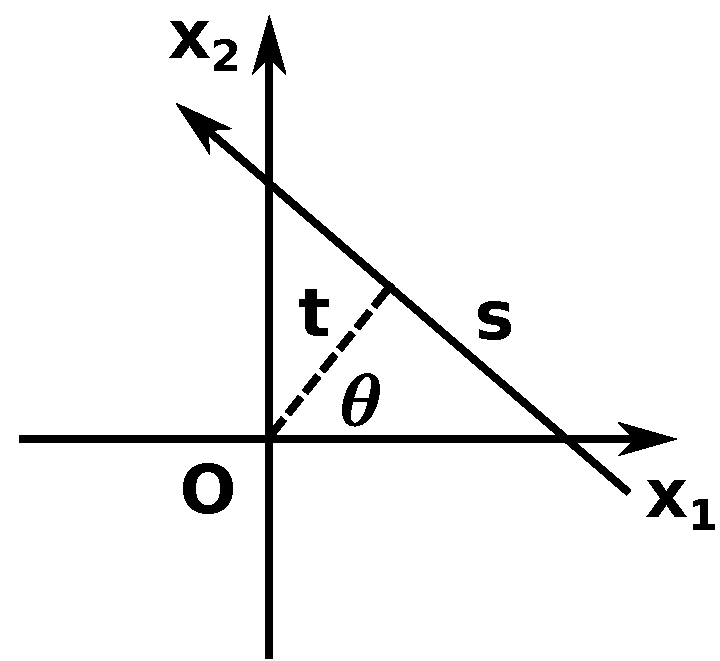
\includegraphics[width=0.38\textwidth]{images/introduction_radon_transform_refsystem.pdf}
  \end{center}
  \caption[Reference system.]{Reference system for formula (\ref{radon_transform_8}).}
  \label{introduction:radon-transform:reference-system}
\end{figure}
The slant stacking approximation of the discrete Radon transform divides the interval $[0,\pi]$
in two regions: one for nearly-horizontal lines $\theta \leq \pi/4$ and $3\pi/4 \leq \theta \leq \pi$;
one for nearly-vertical lines $\pi/4 \leq \theta \leq 3\pi/4$. The slant stacking 
approximation with nearest neighbor interpolation 
results \cite{Toft1996}:
\begin{equation}
    \Radon\{f\}\left[\theta_{k},t_{j}\right] = \begin{cases}
                                                \displaystyle \frac{\Delta x_{1}}{|\sin\theta_{k}|} \sum\limits_{m}f\left[x_{1,m},\lfloor ax_{1,m}+b \rceil\right] 
                                                 & \text{for} \hspace{0.2cm}|\sin\theta| > \frac{\sqrt{2}}{2}\\[1em]
                                                \displaystyle \frac{\Delta x_{2}}{|\cos\theta_{k}|} \sum\limits_{n}f\left[\lfloor a'x_{2,n}+b'\rceil,x_{2,n}\right] 
                                                 & \text{for} \hspace{0.2cm}|\sin\theta| \leq \frac{\sqrt{2}}{2} 
                                               \end{cases}\hspace{0.3cm},
  \label{radon_transform_9}
\end{equation}
where $x_{1,m} = x_{1}^{\text{min}} + m\Delta x_{1}$ for $m = 0, 1, ..., M-1 \in \mathbb{N}$, 
$x_{2,n} = x_{2}^{\text{min}} + n\Delta x_{2}$ for $n = 0, 1, ..., N-1 \in \mathbb{N}$,
$\lfloor...\rceil$ represents the operator rounding to the next integer and
\begin{equation}
\begin{split}
  & a = -\frac{\Delta x_{1}}{\Delta x_{2}}\frac{\cos\theta}{\sin\theta} \hspace{1cm} b = \frac{t - x_{1}^{\text{min}}\cos\theta 
         - x_{2}^{\text{min}}\sin\theta}{\Delta x_{2}\sin\theta} \\[1em]
  & a' = \frac{1}{a} \hspace{2.5cm} b' = \frac{t - x_{1}^{\text{min}}\cos\theta 
         - x_{2}^{\text{min}}\sin\theta}{\Delta x_{1}\cos\theta} \hspace{0.3cm}.
  \label{radon_transform_10}       
\end{split}  
\end{equation}
Formula (\ref{radon_transform_9}) clearly shows that interpolation is needed only along the $s$-direction,
being $x_{1}$ or $x_{2}$ depending on the selected $\theta$. The slant stacking approximation
with linear interpolation becomes \cite{Toft1996}:
\begin{equation}
    \hspace*{0cm}\Radon\{f\}\left[\theta_{k},t_{j}\right] = \begin{cases}
                                                \displaystyle \frac{\Delta x_{1}}{|\sin\theta_{k}|} \sum\limits_{m}(1-\omega)f\left[x_{1,m},\lfloor ax_{1,m}+b \rfloor\right] 
                                                 + \omega f\left[x_{1,m},\lfloor ax_{1,m}+b \rfloor + 1\right] \\[-0.1em] \hspace{7.2cm} \text{for} \hspace{0.2cm}|\sin\theta| > \frac{\sqrt{2}}{2}\\[1em]
                                                \displaystyle \frac{\Delta x_{2}}{|\cos\theta_{k}|} \sum\limits_{n}(1-\omega')f\left[\lfloor a'x_{2,n}+b'\rfloor,x_{2,n}\right] 
                                                 + \omega' f\left[\lfloor ax_{2,m}+b \rfloor + 1,x_{2,m}\right] \\[-0.1em] \hspace{7.2cm} \text{for} \hspace{0.2cm}|\sin\theta| \leq \frac{\sqrt{2}}{2} 
                                               \end{cases}
  \label{radon_transform_11} 
\end{equation}
where $a, a', b, b'$ are defined in (\ref{radon_transform_10}), $\lfloor...\rfloor$ is the flooring operator,
$\omega = ax_{1,m}+b - \lfloor ax_{1,m}+b\rfloor$ and $\omega' = a'x_{2,n}+b' - \lfloor a'x_{2,n}+b'\rfloor$.
Given a square image $N \times N$ pixels and $N$ views in $[0,\pi]$, the slant slacking implementation of the discrete
radon transform with either nearest neighbor or linear interpolation is characterized by a complexity $\Complexity(N^{3})$.


\subsubsection{Pixel-, ray- and distance-driven projectors}
\label{introduction:radon-transform:driven-approaches}
\begin{figure}[!b]
    \hspace{-1.0cm}
    \subfloat[Pixel-driven approach]{{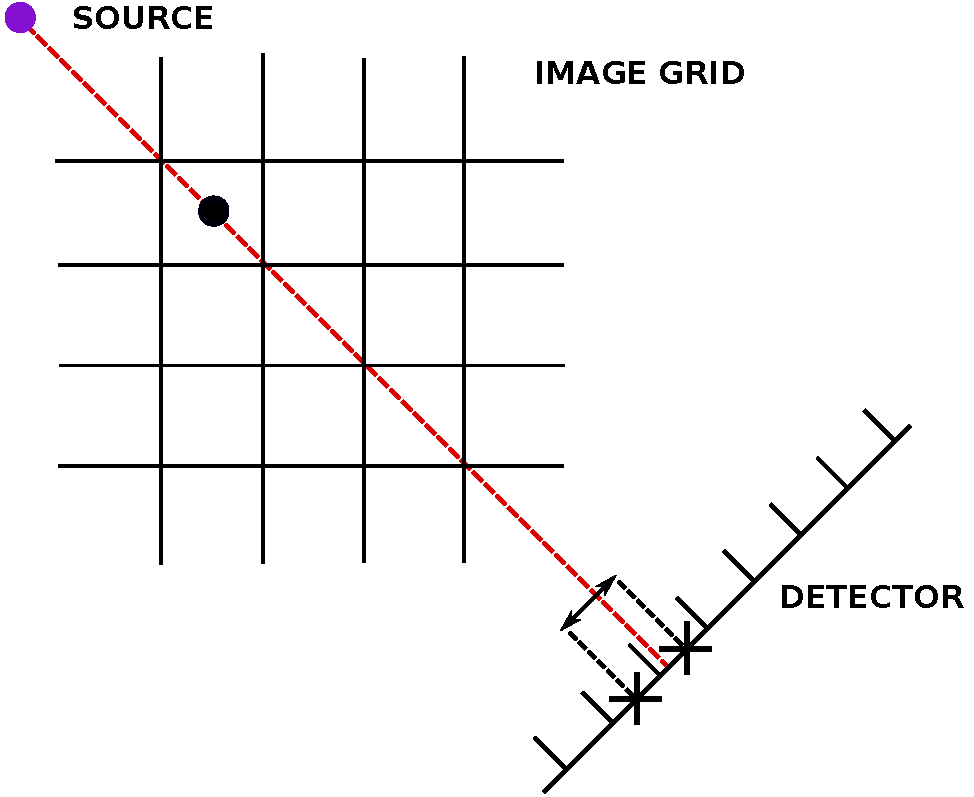
\includegraphics[width=6cm]{images/introduction_radon_transform_pixel_driven.pdf}\label{introduction:radon-transform:pixel} }}%    
    \subfloat[Ray-driven approach]{{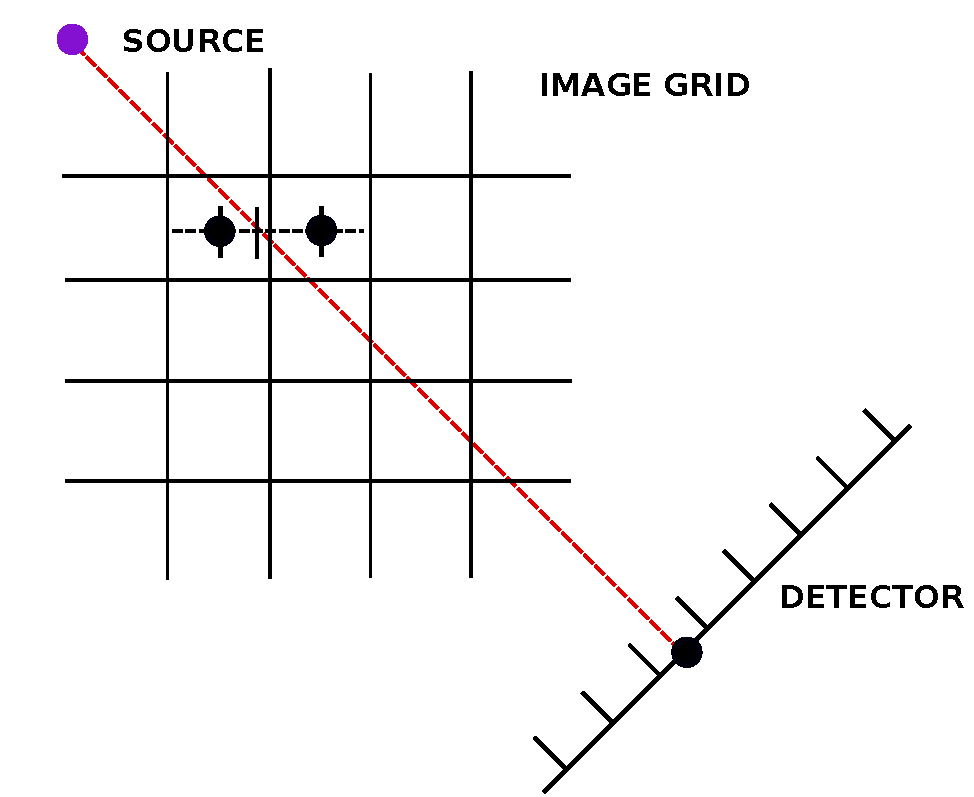
\includegraphics[width=6cm]{images/introduction_radon_transform_ray_driven.pdf}\label{introduction:radon-transform:ray}  }}%
    \subfloat[Distance-driven approach]{{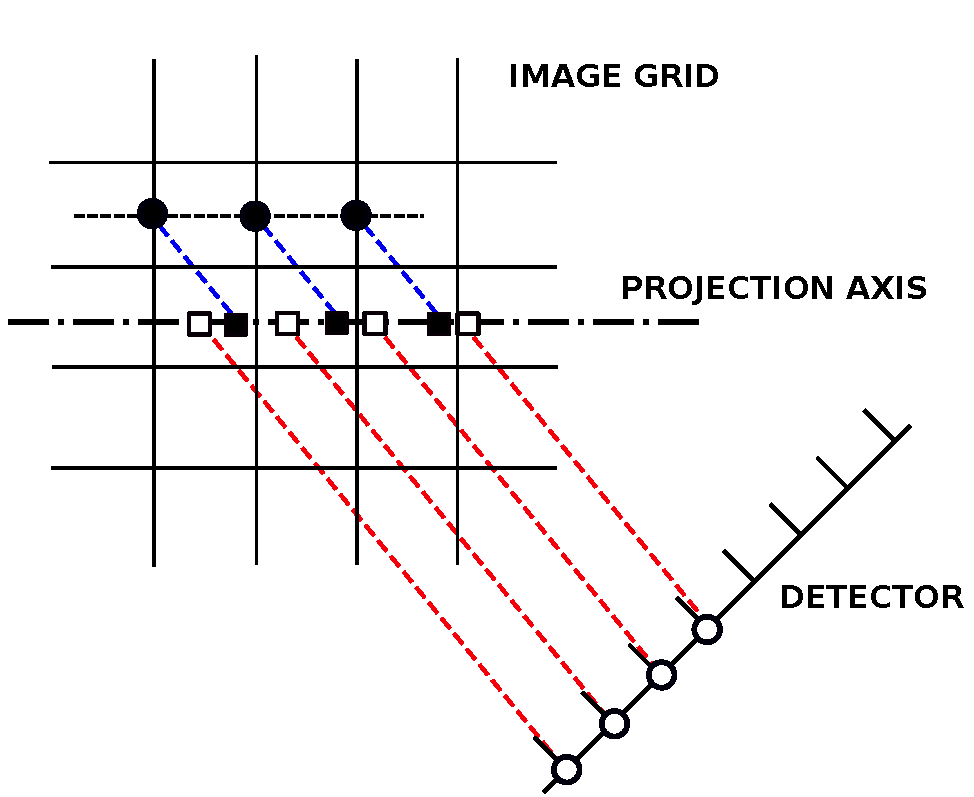
\includegraphics[width=6cm]{images/introduction_radon_transform_distance_driven.pdf}\label{introduction:radon-transform:distance}  }}%    
    \caption[Schematic representation of different forward projectors.]{Schematic representation of the different mechanisms characterizing the pixel-,
              ray- and distance-driven approach for forward projection. 
              This figure is readapted from \cite{Deman2004}.
              }%
    \label{introduction:radon-transform:pixel-ray-distance}%
\end{figure}
In the pixel-driven approach \cite{Herman2009}, the source point is connected to the selected pixel center until intersection
with the detector line, as displayed in Fig. \ref{introduction:radon-transform:pixel}. A linear
interpolation scheme distributes the pixel value to the two detector cells that enclose the ray end point (they are indicated with a cross in Fig. \ref{introduction:radon-transform:pixel}). 
Pixel-driven forward projection is rarely utilized due its characteristic high-frequency artifacts \cite{Zeng1993}.
\newline
The ray-driven approach \cite{Joseph1982} connects the source to the center of a selected detector cell (Fig. \ref{introduction:radon-transform:ray}).
The latter point is projected for each row (column) onto the horizontal (vertical) axis joining the centers of the two image pixels, that surround the ray (this axis
is represented in Fig. \ref{introduction:radon-transform:ray} as a dashed horizontal line within the image grid): 
a linear interpolation scheme weighs the contributions for each couple of image pixels. The ray-driven projection suffers from the same kind of high-frequency 
artifacts affecting the pixel-driven approach \cite{DeMan2002}.
\newline
The distance-driven approach \cite{DeMan2002,Deman2004} in Fig. \ref{introduction:radon-transform:distance}
projects the pixel boundaries (black dots) of each image row/column and
the detector cell boundaries (white dots) onto a common axis
(this axis
is represented in Fig. \ref{introduction:radon-transform:distance} as a dashed horizontal line within the image grid).
The overlap between the interval defined by the projected boundaries of an image pixel (black squares)
and the one defined by the projected boundaries
of a detector cell (white squares) weighs the contribution of the selected image pixel to the selected detector cell (and vice versa).
This method differs substantially from the pixel- and ray-driven
approaches for two reasons:
(i) the distance-driven strategy is faster, as the main loop runs over the projected boundaries on the projection axis,
rather than running over the image pixels or detector cells; (ii) 
the linear interpolation scheme is replaced with the calculation of overlapping intervals. This different approach prevents projections
from being affected by the aforementioned high-frequency artifacts \cite{DeMan2002,Deman2004}.


\subsubsection{Alternative basis for image representation}
The previous implementations of the Radon transform employ the most common basis for image representation:
an array of abutting square pixels (cubic voxels, if the 3D case is considered).
This basis function assumes that each pixel has unit value inside and is zero outside. The 
major drawback of a pixel basis is that combinations of such piecewise-constant
elements may represent a rather poor approximation of smoothly varying functions.
\newline
Given an image $\mathbf{f} \in \mathbb{R}^{M,N}$ sampled at nodes of a square grid 
$G = \{\, \forall \, \mathbf{x} \in \mathbb{R}^{2}\; |\; \mathbf{x} = \mathbf{x}_{m,n} = \mathbf{x}_{0} + (m,n)^{T}\;,\; m = 1, 2, ..., M \;,\; n = 1, 2, ..., N\}$
and a generic set of functions $\Phi_{q}\::\:\mathbb{R}^{2} \longrightarrow
\mathbb{R}$, the continuous representation of the image on the selected basis results:
\begin{equation}
  \tilde{f}(\mathbf{x}) = \sum\limits_{q=1}^{Q} c_{q}\:\Phi_{q}(\mathbf{x})\;\;,\;\;\forall\:\mathbf{x} \in \mathbb{R}^{2} 
  \hspace{0.4cm}\text{such that}\hspace{0.3cm}\tilde{f}(\mathbf{x}_{m,n} ) = f_{m,n}\hspace{0.3cm},
\label{introduction:radon-transform:alternative-basis-1}
\end{equation}
where $c_{q}$'s are the basis coefficients. Due to linearity of the Radon transform, it follows that:
\begin{equation}
  p\left[\theta_{k},t_{j}\right] \cong \Radon\left\{ \sum\limits_{q=1}^{Q} c_{q}\:\Phi_{q}(\mathbf{x}) \right\}
     = \sum\limits_{q=1}^{Q} c_{q}\:\Radon\left\{\Phi_{q}(\mathbf{x}) \right\} \hspace{0.3cm},
\label{introduction:radon-transform:alternative-basis-2}     
\end{equation}
where $\left[\theta_{k},t_{j}\right]$ refers to the discrete projection points of $\mathbf{f}$. 
Once $\Phi_{q}(\mathbf{x})$ are chosen, $\Radon\left\{\Phi_{q}(\mathbf{x}) \right\}$ is determined regardless
of the object under study (the object information is entirely encoded by the coefficients  $c_{q}$'s).
\newline
According to \cite{Lewitt1990}, the optimal $\Phi_{q}(\mathbf{x})$ has to be smooth
and both space- and band-limited. If the basis functions are space-limited, the computation of $\tilde{f}(\mathbf{x})$ can be 
performed very efficiently. Requiring the basis function to be band-limited has to do with the finite nature of the data
(one should not retrieve frequencies above the band limit of the data)
and with the null space of the Radon transform. It has been shown that the functions living in the null space
of the Radon transform (known as
\textit{ghosts}) have Fourier transform characteristics complementary to those of band-limited functions \cite{Louis1984}.
In the field of signal processing, functions limited in some space are also called \textit{windows}.
\newline 
A window easy to compute and being (nearly) optimally concentrated in real and Fourier domain is the Kaiser-Bessel \cite{Kaiser1966}:
\begin{equation}
  \Phi_{q}^{(l)}(r) = \begin{cases}
		     \displaystyle \frac{\left(\sqrt{1-\left(\frac{r}{a}\right)^{2}}\right)^{m}\:I_{l}\left(\alpha\sqrt{1-\left(\frac{r}{a}\right)^{2}}\right)}{I_{l}(\alpha)} & 0 \leq r \leq a\\
		     0 & \text{otherwise}
                \end{cases} \hspace{0.3cm},
\label{introduction:radon-transform:alternative-basis-3}                
\end{equation}
where $I_{l}$ denotes the $l$-th order modified Bessel function of the first kind, $a$ is the support radius
and $\alpha$ is the tapering parameter, controlling the trade-off between the width of the main lobe
and the amplitude of the side lobes of the Fourier transform of the function. Since the Kaiser-Bessel window
(\ref{introduction:radon-transform:alternative-basis-3}) is a radially symmetric function, the expression of
its Radon transform does not depend on $\theta$ \cite{Lewitt1990}:
\begin{equation}
  \Radon\left\{\Phi_{q}^{l}(r)\right\}(t) = \frac{a}{I_{l}(\alpha)} \left(\frac{2\pi}{\alpha}\right)^{\frac{1}{2}}
  I_{l+1/2}\left(\alpha\sqrt{2-\left(\frac{t}{a}\right)^{2}}\right) \left[\sqrt{1-\left(\frac{t}{a}\right)^{2}}\right]^{l+1/2}\hspace{0.3cm}.
\end{equation}
Another basis recently introduced for tomographic image reconstruction is the tensor-product B-spline \cite{Horbelt2002},
that has shown potential particularly for the case of DPC data \cite{Nilchian2013}.
Defining $\Delta_{h}^{n}f(x)$ the $n$-fold iteration of the finite difference operator 
$\Delta_{h}f(x) = \left( f(x+h/2) - f(x-h/2) \right) / h$ and $x_{+} = \text{max}\{0,x\}$, $\beta^{(l)}$
is a centered univariate B-spline of degree $l$:
\begin{equation}
  \beta^{(l)}(x) = \frac{\Delta_{1}^{l+1}}{l!} x_{+}^{l}\hspace{0.3cm}.
\end{equation}
In this case, $\Phi_{q}^{(l)}(\mathbf{x}) = \beta^{(l)}(x_{1})\beta^{(l)}(x_{2})$ and the expression of the $n$-th derivative of the 
Radon transform is \cite{Horbelt2002,Nilchian2013}:
\begin{equation}
  \Radon^{(n)}\left\{\Phi_{q}^{(l)}(\mathbf{x})\right\}(\theta,t) = \frac{\Delta_{\cos\theta}^{l+1}\:\Delta_{\sin\theta}^{l+1}}{(2l-n+1)}\,
  t_{+}^{2l-n+1} \hspace{0.3cm}.
\end{equation}


\subsection{Parallel beam geometry}
\label{introduction:radon-transform:geometry}
 All the techniques developed and/or analyzed in this work address the reconstruction of tomographic data in parallel beam geometry (PBG),
 The assumption is that X-rays are traveling parallel to each other
on planes perpendicular to the rotation axis $r$. This allows to greatly simplify the X-ray projection model, since the contribution to
the forward projection at a certain height $\bar{r}$ originates from the object information lying on the plane perpendicular to
the $r$-axis and intersecting it at $(0,0,\bar{r})$. Each 2D projection can, therefore, be regarded as a stack of independent projection lines
being perpendicular to $r$. The ensemble of 1D projections at a fixed height collected in $[0,\pi)$ is called \emph{sinogram}.
Fig. \ref{introduction:radon-transform:sinogram} is an example of a sinogram, whose projections are stacked along the vertical axis
(namely, the ``view direction''; the horizontal axis is also called ``channel direction'').
\begin{figure}[!h]
    \centering
    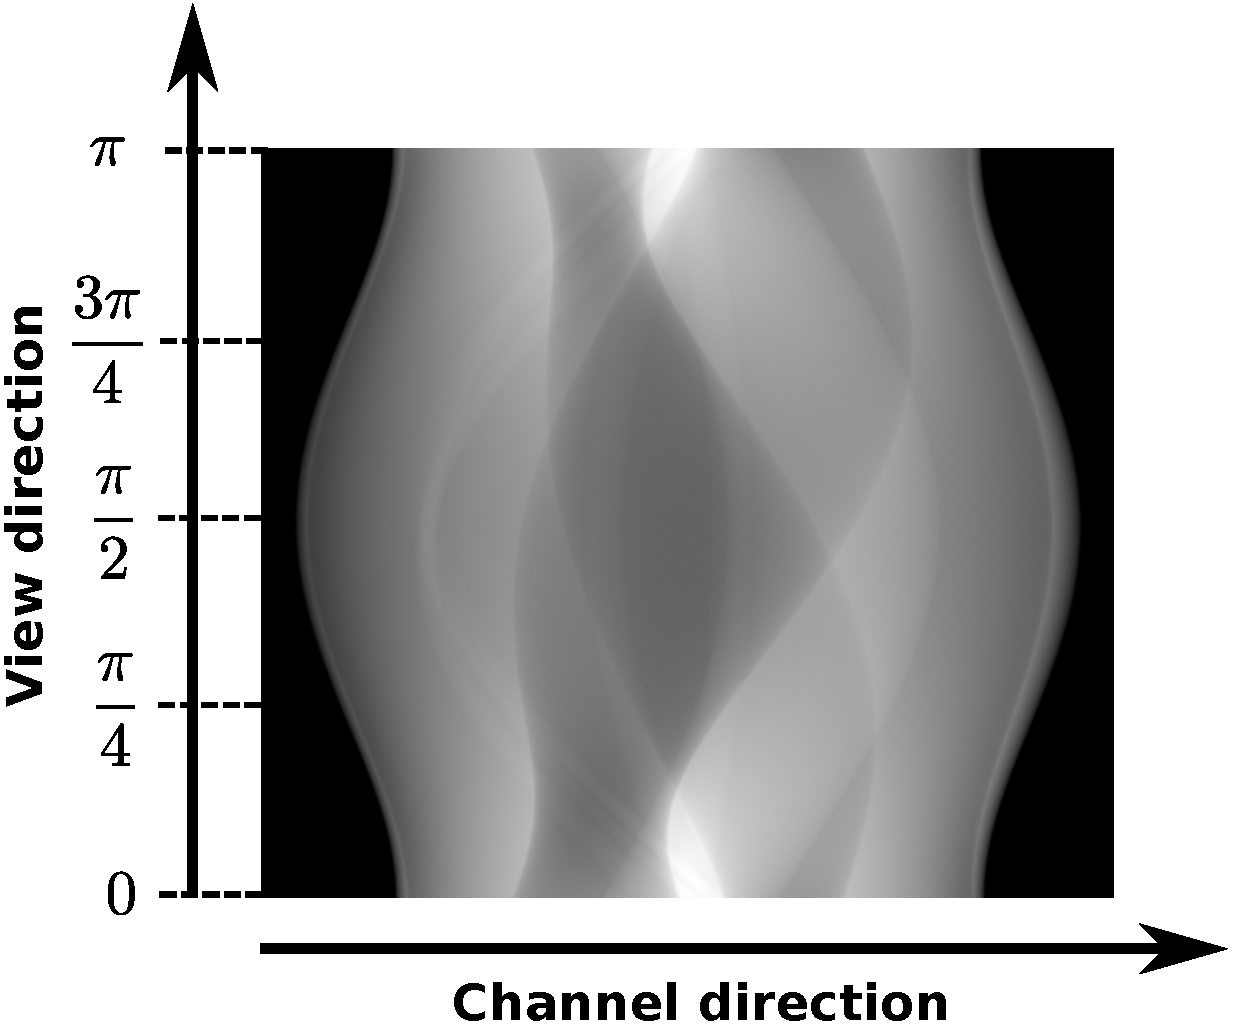
\includegraphics[width=7cm]{images/introduction_radon_transform_sinogram.pdf}   
   \caption[Example of a sinogram.]{Example of a sinogram.}
    \label{introduction:radon-transform:sinogram}
\end{figure}

\section{Analytical reconstruction}
\subsection{Fourier slice theorem}
\label{subsection:fourier-slice-theorem}
The Fourier slice theorem (FST) states that
the 1D Fourier transform of a projection line acquired at angle $\theta$ with respect to a certain axis corresponds to the 2D Fourier transform 
of the object, sampled along a line that forms the same angle with respect to the same axis \cite{Kak2001}.
In mathematical terms, it means that:
\begin{equation}
  \Four_{t}\left\{\Radon\left\{ f \right\}\right\}(\theta,\omega) = 
  \Four_{x_{1},x_{2}}\left\{ f \right\}\left(u_{1},u_{2}\right)
  \Bigr\rvert_{\substack{u_{1} = \omega\cos\theta\\u_{2} = \omega\sin\theta}}\hspace{0.3cm},
  \label{introduction:analytical-reconstruction:fourier-slice-theorem}
\end{equation}
where
\begin{equation}
\begin{split}
    & \Four_{t}\left\{\Radon\left\{ f \right\}\right\}(\theta,\omega) =
	\int\limits_{-\infty}^{+\infty}dt\:\Radon\left\{ f \right\}(\theta,t)\:\exp\left(-2\pi i\omega t\right) \hspace{0.3cm},\\
    & \Four_{x_{1},x_{2}}\left\{ f \right\}\left(u_{1},u_{2}\right) =
	\int\limits_{-\infty}^{+\infty}dx_{1} \int\limits_{-\infty}^{+\infty}dx_{2} f\left(x_{1},x_{2}\right) 
	    \:\exp\left(-2\pi i\left(x_{1}u_{1} + x_{2}u_{2}\right)\right)\hspace{0.3cm}.
\end{split}
\end{equation}
The derivation (\ref{introduction:analytical-reconstruction:fourier-slice-theorem}) makes use of expression (\ref{radon_transform_8})
of the Radon transform and of the coordinate change from $(t,s)$ to $(x_{1},x_{2})$ \cite{Kak2001}:
\begin{equation}
    \begin{split}
    \Four_{t}\left\{\Radon\left\{ f \right\}\right\}(\theta,\omega) &= 
             \int\limits_{-\infty}^{+\infty}dt\:\Radon\left\{ f \right\}(\theta,t)\:\exp\left(-2\pi i\omega t\right)                        
             = \int\limits_{-\infty}^{+\infty}dt\:\left( \int\limits_{-\infty}^{+\infty}ds\:f(t,s) \right)\:\exp\left(-2\pi i\omega t\right)\\  
                                                                         &=
             \int\limits_{-\infty}^{+\infty}dx_{1}\int\limits_{-\infty}^{+\infty}dx_{2}\:f\left(x_{1},x_{2}\right)
                          \:\exp\left(-2\pi i\omega\left(x_{1}\cos\theta + x_{2}\sin\theta\right)\right) \\
                                                                         &=
                          \Four_{x_{1},x_{2}}\left\{ f \right\}\left(\omega\cos\theta,\omega\sin\theta\right)\hspace{0.3cm}.
    \end{split} \hspace{0.3cm}.
\end{equation}
Equation (\ref{introduction:analytical-reconstruction:fourier-slice-theorem}) clearly shows that sampling the 1D Fourier
transform of a projection line is equivalent to sampling the 2D Fourier transform of the object
in a polar fashion. Theoretically speaking, the reconstruction of $f$ demands the following three steps: (i) acquisition of
an infinite number of projections in $[0,\pi)$; (ii)
1D Fourier transform of the projections; (iii) 2D inverse Fourier transform.
In practice, implementing such an approach is not so trivial, because the 2D Fourier space of the object is sampled
in a polar fashion by the 1D FFT-transformed projections and it is necessary to interpolate those samples on a Cartesian grid
to apply the IFFT 2D. Fourier methods for tomographic reconstruction are treated in detail in Chapter \ref{chapter:gridding-projectors}.
%
%
%
\subsection{Filtered backprojection}
Filtered backprojection (FBP) is a reconstruction algorithm that descends directly from the FST.
% The derivation of the FBP formula in \cite{Kak2001} starts with an identity and carries the following steps on the right hand side:
substitution with polar coordinates; split of the integral in two parts, one where $\theta \in [0,\pi/2]$, the other where
$\theta \in [\pi/2,\pi]$; transformation of the second integral; recomposition of the two integrals to form again a single one;
application of property \ref{radon_transform_3}; utilization of the FST.
\begin{align}
\allowdisplaybreaks[2]
    f\left(x_{1},x_{2}\right) &= \int\limits_{-\infty}^{+\infty}du_{1}\int\limits_{-\infty}^{+\infty}du_{2}\:\Four\{f\}\left(u_{1},u_{2}\right)
	\:\exp\left(-2\pi i\left(x_{1}u_{1} + x_{2}u_{2}\right)\right) \nonumber \\
	                      &= \int\limits_{0}^{2\pi}d\theta \underbrace{\int\limits_{0}^{+\infty} d\omega \: \omega\: \Four\{f\}\left(\theta,\omega\right)
	\:\exp\left(-2\pi i\omega\left(x_{1}\cos\theta + x_{2}\sin\theta\right)\right)}_{:= D} = \int\limits_{0}^{\pi}d\theta\: D + \int\limits_{\pi}^{2\pi}d\theta\: D \nonumber \\
	                      &= \int\limits_{0}^{\pi}d\theta\: D + 
\underset{\text{substituted } \theta' = \theta - \pi}{\int\limits_{0}^{\pi}d\theta'\int\limits_{0}^{+\infty} d\omega\:\omega \: \Four\{f\}\left(\theta'+\pi,\omega\right)\:\exp\left(+2\pi i\omega\left(x_{1}\cos\theta' + x_{2}\sin\theta'\right)\right)} \nonumber \\
	                      &= \int\limits_{0}^{\pi}d\theta \: D + 
    \int\limits_{0}^{\pi}d\theta'\:\int\limits_{0}^{+\infty} d\omega\:\omega\:\underbrace{\Four\{f\}\left(\theta',-\omega\right)}_{\text{used property (23)}}\:\exp\left(+2\pi i\omega\left(x_{1}\cos\theta' + x_{2}\sin\theta'\right)\right) \nonumber \\
			      &= \int\limits_{0}^{\pi}d\theta \: D + 
    \underset{\text{substituted } \omega' = -\omega\;\;\text{and used again both } \theta\;,\;\omega}{\int\limits_{0}^{\pi}d\theta\int\limits_{-\infty}^{0} d\omega'\:(-\omega') \: \Four\{f\}\left(\theta,\omega'\right)\:\exp\left(-2\pi i\omega'\left(x_{1}\cos\theta + x_{2}\sin\theta\right)\right)} \nonumber \\
			      &= \int\limits_{0}^{\pi}d\theta\int\limits_{-\infty}^{+\infty} d\omega\:|\omega| \: \underbrace{\Four\{f\}\left(\theta,\omega\right)}_{\text{apply FST}}\:\exp\left(-2\pi i\omega\left(x_{1}\cos\theta + x_{2}\sin\theta\right)\right) \nonumber \\
                              &= \int\limits_{0}^{\pi}d\theta\int\limits_{-\infty}^{+\infty} d\omega\:|\omega| \: \Four_{t}\left\{\Radon\{f\}\right\}\left(\theta,\omega\right)\:\exp\left(-2\pi i\omega\left(x_{1}\cos\theta + x_{2}\sin\theta\right)\right) 
                                  \label{introduction:analytical-reconstruction:fbp1}\\
                              &= \int\limits_{0}^{\pi}d\theta\:\Four^{-1}\left\{|\omega|\right\}(t) \ast \Radon\{f\}(\theta,t) \hspace{0.2cm},\;\;\text{with} \hspace{0.2cm} t = x_{1}\cos\theta + x_{2}\sin\theta
                                  \label{introduction:analytical-reconstruction:fbp2} \\                            
                              &= \int\limits_{0}^{\pi}d\theta\int\limits_{-\infty}^{+\infty} dt'\:\Four^{-1}\left\{|\omega|\right\}(t-t') \: \Radon\{f\}(\theta,t') \hspace{0.3cm},
                                  \nonumber
\end{align}
where $\ast$ is the convolution operator. The passage from (\ref{introduction:analytical-reconstruction:fbp1}) to
(\ref{introduction:analytical-reconstruction:fbp2}) is made possible by the convolution property of the Fourier transform,
namely, $f \ast g = \Four^{-1}\{ \Four\{ f \} \Four\{ g \} \}$.
(\ref{introduction:analytical-reconstruction:fbp1}) and (\ref{introduction:analytical-reconstruction:fbp2})
are equivalent continuous formulas of FBP. The difference lies in the inner integral corresponding to the \emph{filtering} step,
which is performed in Fourier domain for the first formula and in the real domain for the second one. The outer integral corresponds
to the \emph{backprojection} step.
\newline
The discretized form of (\ref{introduction:analytical-reconstruction:fbp2}), for example, is:
\begin{equation}
\begin{split}
  f\left[x_{1,m},x_{2,n}\right] &= \Delta\theta\Delta t \sum\limits_{k=0}^{K-1} \; \sum\limits_{j=-J/2}^{J/2-1} \Four^{-1}\{|\omega|\}
                  \left[x_{1,m}\cos\theta_{k} + x_{2,n}\sin\theta_{k} - t_{j}'\right] \ast \Radon\{f\}\left[\theta_{k},t_{j}'\right] \\
                  &= \Delta\theta\Delta t \sum\limits_{k=0}^{K-1} p^{(f)}\left[ x_{1,m}\cos\theta_{k} + x_{2,n}\sin\theta_{k} \right] \hspace{0.3cm},
\end{split}
\label{introduction:analytical-reconstruction:fbp3}
\end{equation}
where $p^{(f)}$ indicates the filtered projection and $\Delta\theta = \pi/K$ provided that the projectons are acquired at equispaced angular intervals.
Generally, the argument of $p^{(f)}$ in (\ref{introduction:analytical-reconstruction:fbp3}) does not exactly
coincide with the center of a detector cell and, therefore, an interpolation scheme is required.
\newline
One of the reasons why FBP has become a broadly adopted reconstruction algorithm for CT since its introduction 
(and for several decades since) is that interpolation is performed entirely in the real domain, differently from the Fourier
methods briefly mentioned in \ref{subsection:fourier-slice-theorem}. Interpolation errors in the real domain are localized
in a neighborhood; interpolation errors in the Fourier domain are smeared back onto the entire image, once the 
inverse Fourier transform is computed. Considered an image $\mathbf{f} \in \mathbb{R}^{M\times N}$ and
its discrete Fourier transform (DFT) $\mathbf{\hat{f}}$, an error in Fourier domain can be thought as an impulse 
located at $(\bar{j},\bar{k})$ and added to $\mathbf{\hat{f}}$:
\begin{align}
  \tilde{f}[m,n] &= \sum\limits_{j=0}^{M} \sum\limits_{k=0}^{N} \exp\left( 2\pi ijm/M \right) \: \exp\left( 2\pi ikn/N \right)					      
       \left( \hat{f}\left[j,k\right]
       + a\delta\left[ j - \bar{j} , k - \bar{k} \right] \right) \nonumber\\
       &= f[m,n] + a\:\exp\left( 2\pi i\bar{j}m/M \right)\:\exp\left( 2\pi i\bar{k}n/N \right)\nonumber\\
       &\underset{\text{neglecting the imaginary part}}{\sim f[m,n] + a\cos\left(2\pi * \left(\frac{\bar{j}m}{M} + \frac{\bar{k}n}{N} \right)\right)}\hspace{0.3cm}. 
\label{introduction:analytical-reconstruction:fbp4}
\end{align}
(\ref{introduction:analytical-reconstruction:fbp4}) clearly shows that the initial impulse located at $(\bar{j},\bar{k})$
is transformed by the IDFT into a perturbation periodically added onto the entire image $\forall\:m = 0,1,...,M-1$ and 
$\forall\:n = 0,1,...,N-1$.


\subsection{Filtering step}
\label{intruduction:analytical-reconstruction:filtering-step}
The filtering step acts separately on each projection, suppressing low frequencies (those closer to the origin of the
Fourier domain), as shown by (\ref{introduction:analytical-reconstruction:fbp1}). The filter function $|\omega|$, coming
from the Jacobian of the polar-Cartesian coordinate transformation, is called \emph{ramp} or \emph{Ram-Lak} \cite{Kak2001}.
\newline
To derive the discretized form of the ramp filter, one has first to assume the projections 
$p_{\theta}[t_{j}] = \Radon\{f\}[\theta,t_{j}]$\footnote{The variable $\theta$ is not indexed here 
to simplify the notation. The discretization of the ramp filter involves exclusively the radial variable, $t$.}
 band-limited with bandwidth $W$,
i.e. $\hat{p}_{\theta}[\omega_{j}] = 0$ if $|\omega_{j}| > W$. 
The \emph{sampling theorem} \cite{Whittaker1935} states that for a sampling period $\tau \leq 1/2W$ it follows \cite{Murrell1996}:
\begin{equation}
  p_{\theta}(t) = \sum\limits_{j=-\infty}^{+\infty} p_{\theta}\left[j\tau\right] \: \sinc\left( 2\pi W(t - j\tau)\right)\hspace{0.3cm},
  \label{introduction:analytical-reconstruction:filtering-step1}
\end{equation}
where $\sinc x := \sin x/x$.
(\ref{introduction:analytical-reconstruction:filtering-step1}) is substituted inside the expression of the filtered projection, $p_{\theta}^{(f)}(t)$, in
(\ref{introduction:analytical-reconstruction:fbp1}), where the integration interval is now limited to $[-W,W]$ \cite{Murrell1996}:
\begin{align}
\allowdisplaybreaks[2]
  p_{\theta}^{(f)}(t) &= \int\limits_{-W}^{+W} d\omega\:|\omega| \: \Four\left\{ p_{\theta}(t) \right\}\:\exp\left(-2\pi i\omega t\right) 
	              = \int\limits_{-W}^{+W} d\omega\:|\omega| \: \left( \int\limits_{-\infty}^{+\infty} dt \: p_{\theta}(t) \: \exp\left(2\pi i\omega t\right) \right) \:\exp\left(-2\pi i\omega t\right) \nonumber\\
	              &= \int\limits_{-W}^{+W} d\omega\:|\omega| \: \left( \int\limits_{-\infty}^{+\infty} dt' \: 
	                        \sum\limits_{j=-\infty}^{+\infty} p_{\theta}\left[j\tau\right] \: \sinc\left( 2\pi W(t' - j\tau)\right)
	                        \: \exp\left(2\pi i\omega t'\right) \right) \:\exp\left(-2\pi i\omega t\right) \nonumber\\ 
	              &= \sum\limits_{j=-\infty}^{+\infty} p_{\theta}\left[j\tau\right] \int\limits_{-W}^{+W} d\omega\:|\omega| \: \underbrace{\left( \int\limits_{-\infty}^{+\infty} dt' \: 
	                        \sinc\left( 2\pi W(t' - j\tau)\right)
	                        \: \exp\left(2\pi i\omega t'\right) \right)}_{:= D} \:\exp\left(-2\pi i\omega t\right) \hspace{0.3cm}. 
  \label{introduction:analytical-reconstruction:filtering-step2}				  
\end{align}
Integral $D$ is related to the Fourier transform of the sinc function given by:
\begin{equation}
  \Four\{\sinc t\}(\omega) = \int\limits_{-\infty}^{+\infty} dt \: \sinc t \: \exp\left( 2\pi i\omega t\right) = \rect(\omega) :=
  \begin{cases}
    0 & |\omega| > 1/2 \\
    1/2 & |\omega| = 1/2 \\
    1 & |\omega| < 1/2 
  \end{cases}\hspace*{0.3cm}.
  \label{introduction:analytical-reconstruction:filtering-step3}
\end{equation}
Using (\ref{introduction:analytical-reconstruction:filtering-step3}) to simplify $D$ and considering the discretized version
of the filtered projection,
(\ref{introduction:analytical-reconstruction:filtering-step2}) becomes \cite{Murrell1996}:
\begin{align}
\allowdisplaybreaks[2]
      p_{\theta}^{(f)}[k\tau] &= \frac{1}{2W} \sum\limits_{j=-\infty}^{+\infty} p_{\theta}\left[j\tau\right] 
                                  \int\limits_{-W}^{+W} d\omega \: |\omega| \: \exp\left( -2\pi i\omega (k\tau-j\tau)\right) \nonumber\\
%%                          
                          &= \frac{1}{2W}\sum\limits_{j=-\infty}^{+\infty} p_{\theta}\left[j\tau\right] \int\limits_{-W}^{+W} d\omega\:|\omega|
                              \: \left(\cos\left( 2\pi \omega (k\tau-j\tau)\right)
                                     - \underbrace{ i \sin\left( 2\pi \omega (k\tau-j\tau) \right)}_{ 
                                 \text{the integral of this function is 0}}\right) \nonumber\\
%%                                 
                          &= \frac{W}{2}p_{\theta}\left[k\tau\right] + \frac{1}{W}\sum\limits_{\substack{j=-\infty\\j\neq k}}^{+\infty} 
                                   p_{\theta}\left[j\tau\right] \int\limits_{0}^{+W} d\omega\:|\omega| \: 
                                   \cos\left( 2\pi \omega (k\tau-j\tau)\right)\nonumber\\
%%                                   
                          &= 2W \left( \frac{1}{4}p_{\theta}\left[k\tau\right] - 
                              \sum\limits_{\substack{j=-\infty\\j-k \in \mathbb{Z}_{o}}}^{+\infty} 
                              \frac{p_{\theta}\left[j\tau\right]}{\pi^{2}(j-k)^{2}}\right)
                            = p_{\theta}\left[j\tau\right] \ast h[j\tau] 
                               \hspace{0.2cm},\hspace{0.2cm} h[j\tau] =\begin{cases}
								    1/4 & j=0 \\
								    0   & j \in \mathbb{Z}_{e}\\
								    -1/j^{2}\pi^{2} & j \in \mathbb{Z}_{o}
                                                                 \end{cases}\hspace{0.3cm},
                                                                 \label{introduction:analytical-reconstruction:filtering-step4}
\end{align}
where $\mathbb{Z}_{o}$ and $\mathbb{Z}_{e}$ are the sets of odd and even integer numbers, respectively.
The filter $h$ and its DFT, $\hat{h}$, are plotted in Fig. \ref{introduction:fbp:ramp-filter}. 
$\hat{h}$ resembles the ramp filter in the continuous formulation of FBP ($|\omega|$) with
the difference that $\hat{h}[0] \neq 0$ (although very small), so that the filtering operation does not suppress
the DC term of the projections \cite{Kak2001}.
\newline
The ramp filter compensates for the non-homogeneous sampling of the Fourier domain \cite{Kak2001}, when dealing with
discrete projections. 
\begin{figure}[!b]
    \hspace{0cm}
    \subfloat[]{{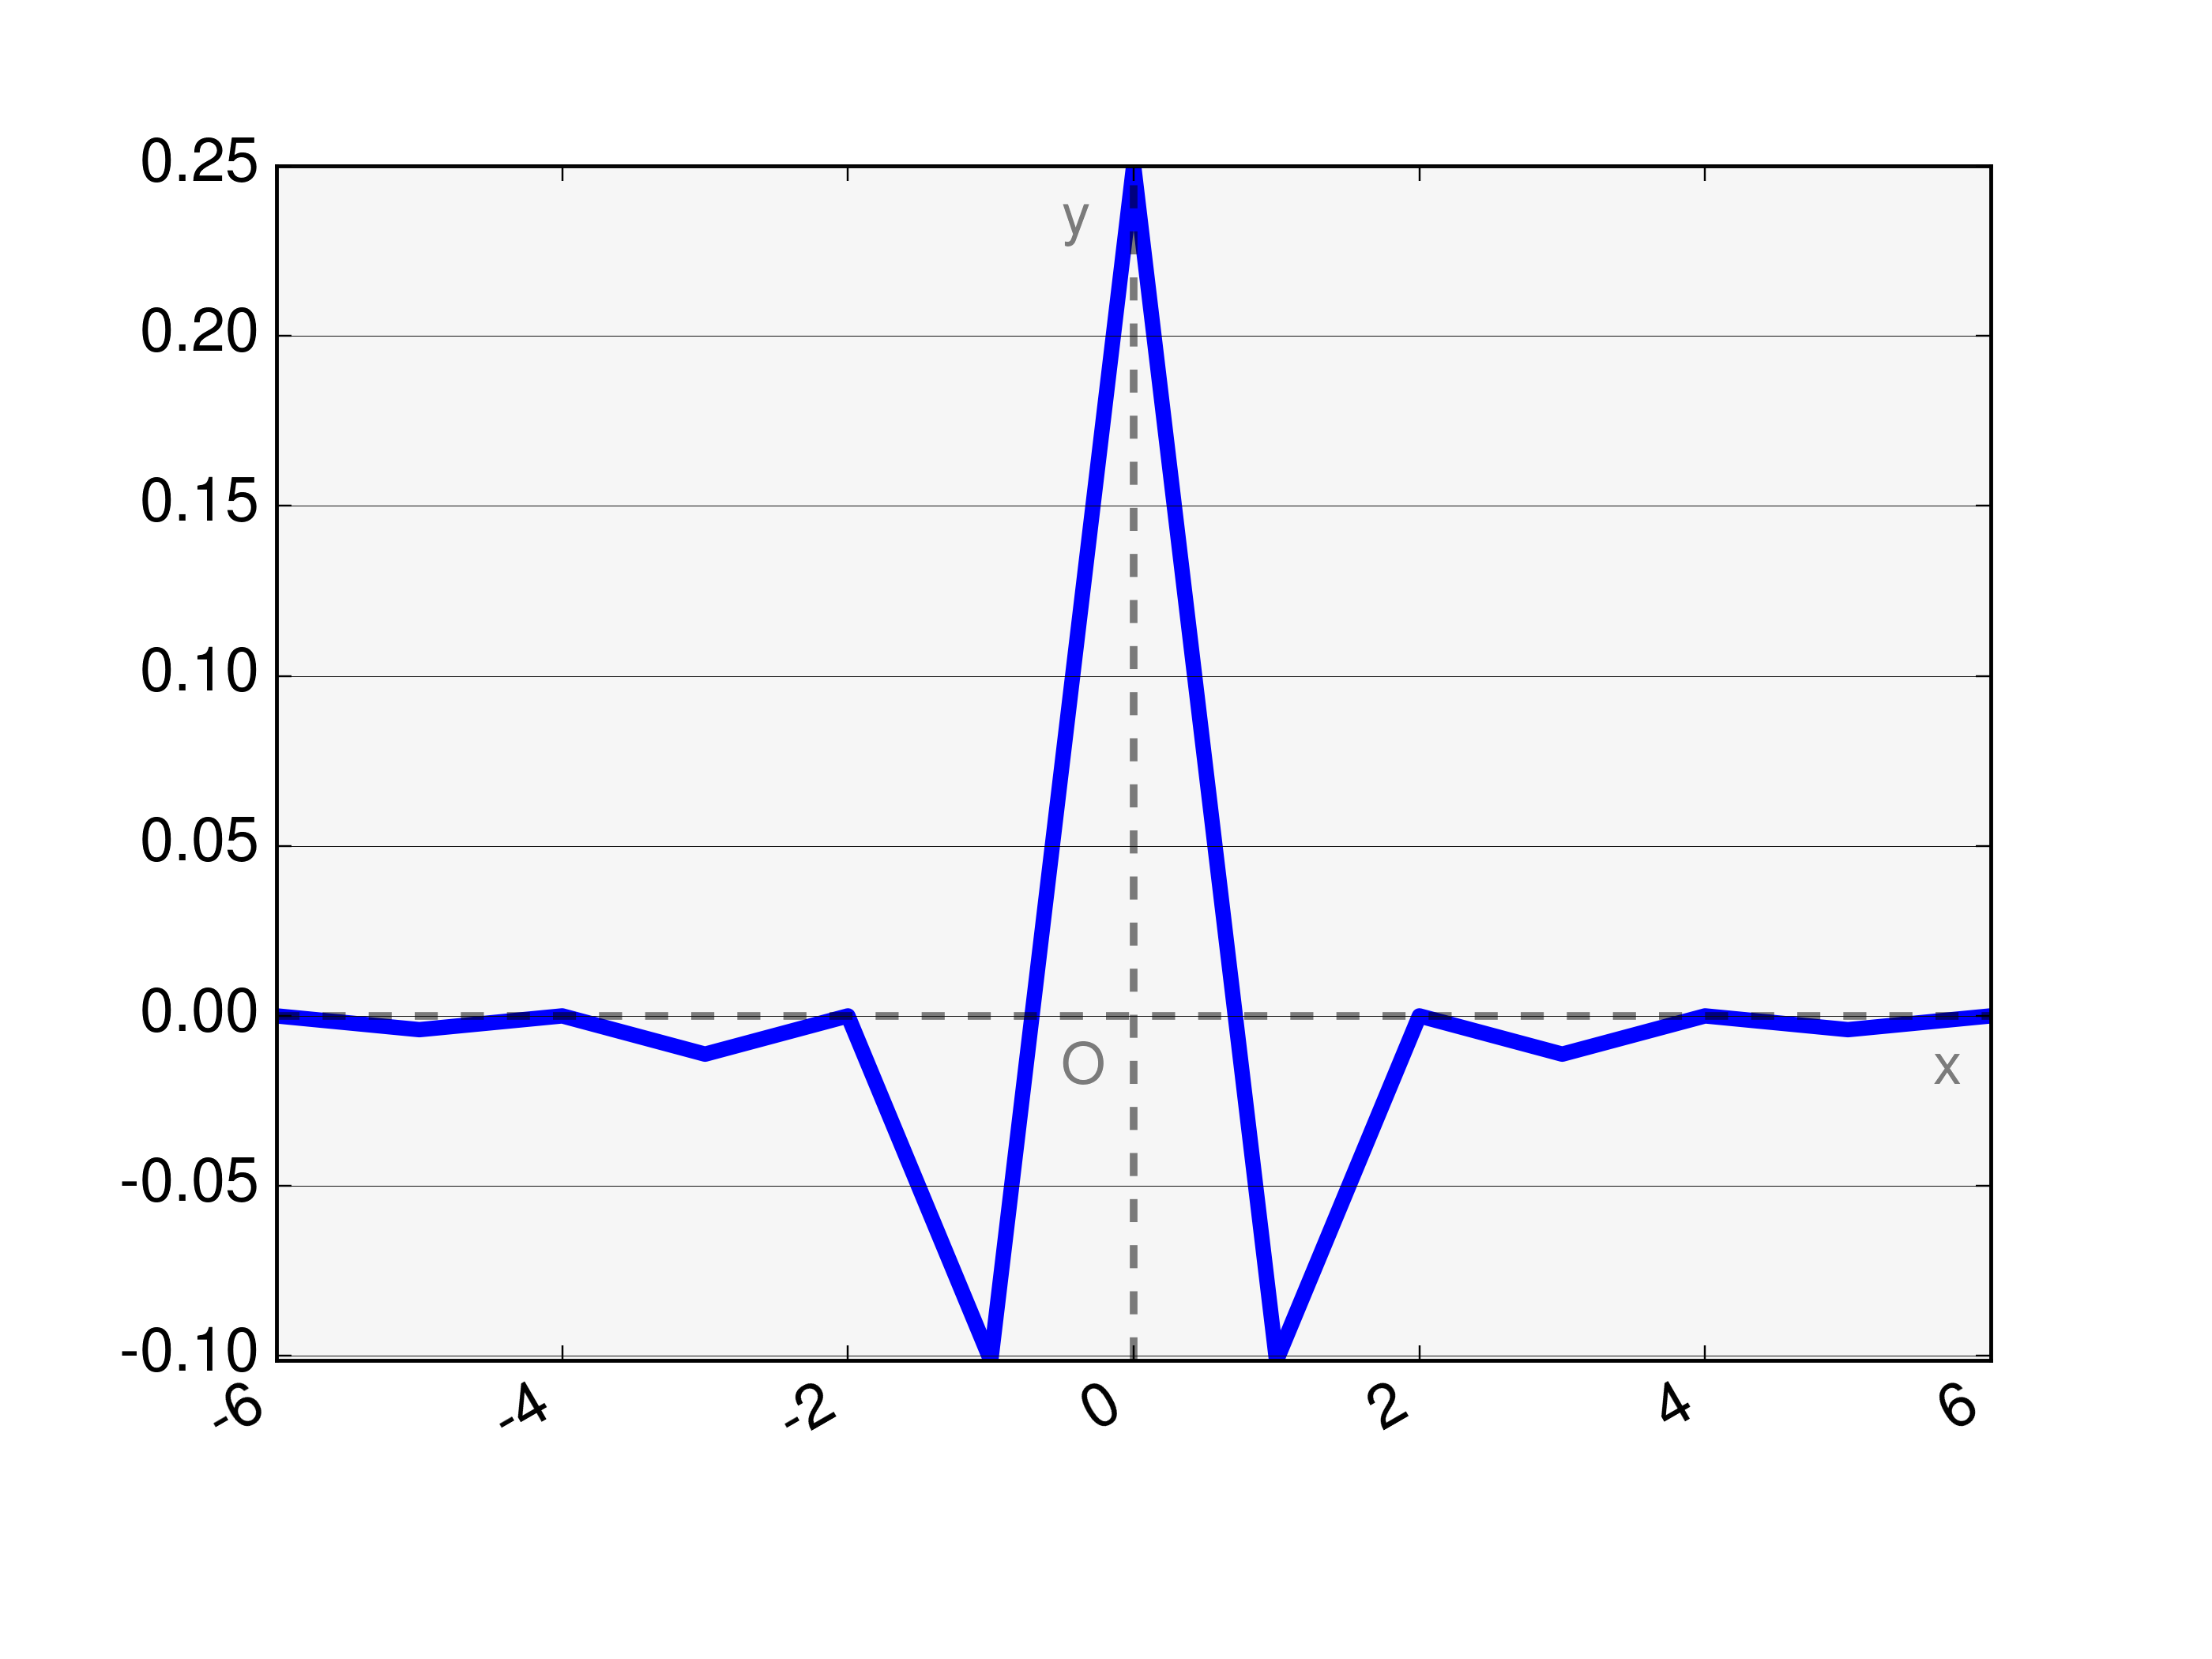
\includegraphics[width=8cm]{images/introduction_fbp_ramp_filter_real_space.png}\label{introduction:fbp:ramp-filter1} }}%    
    \subfloat[]{{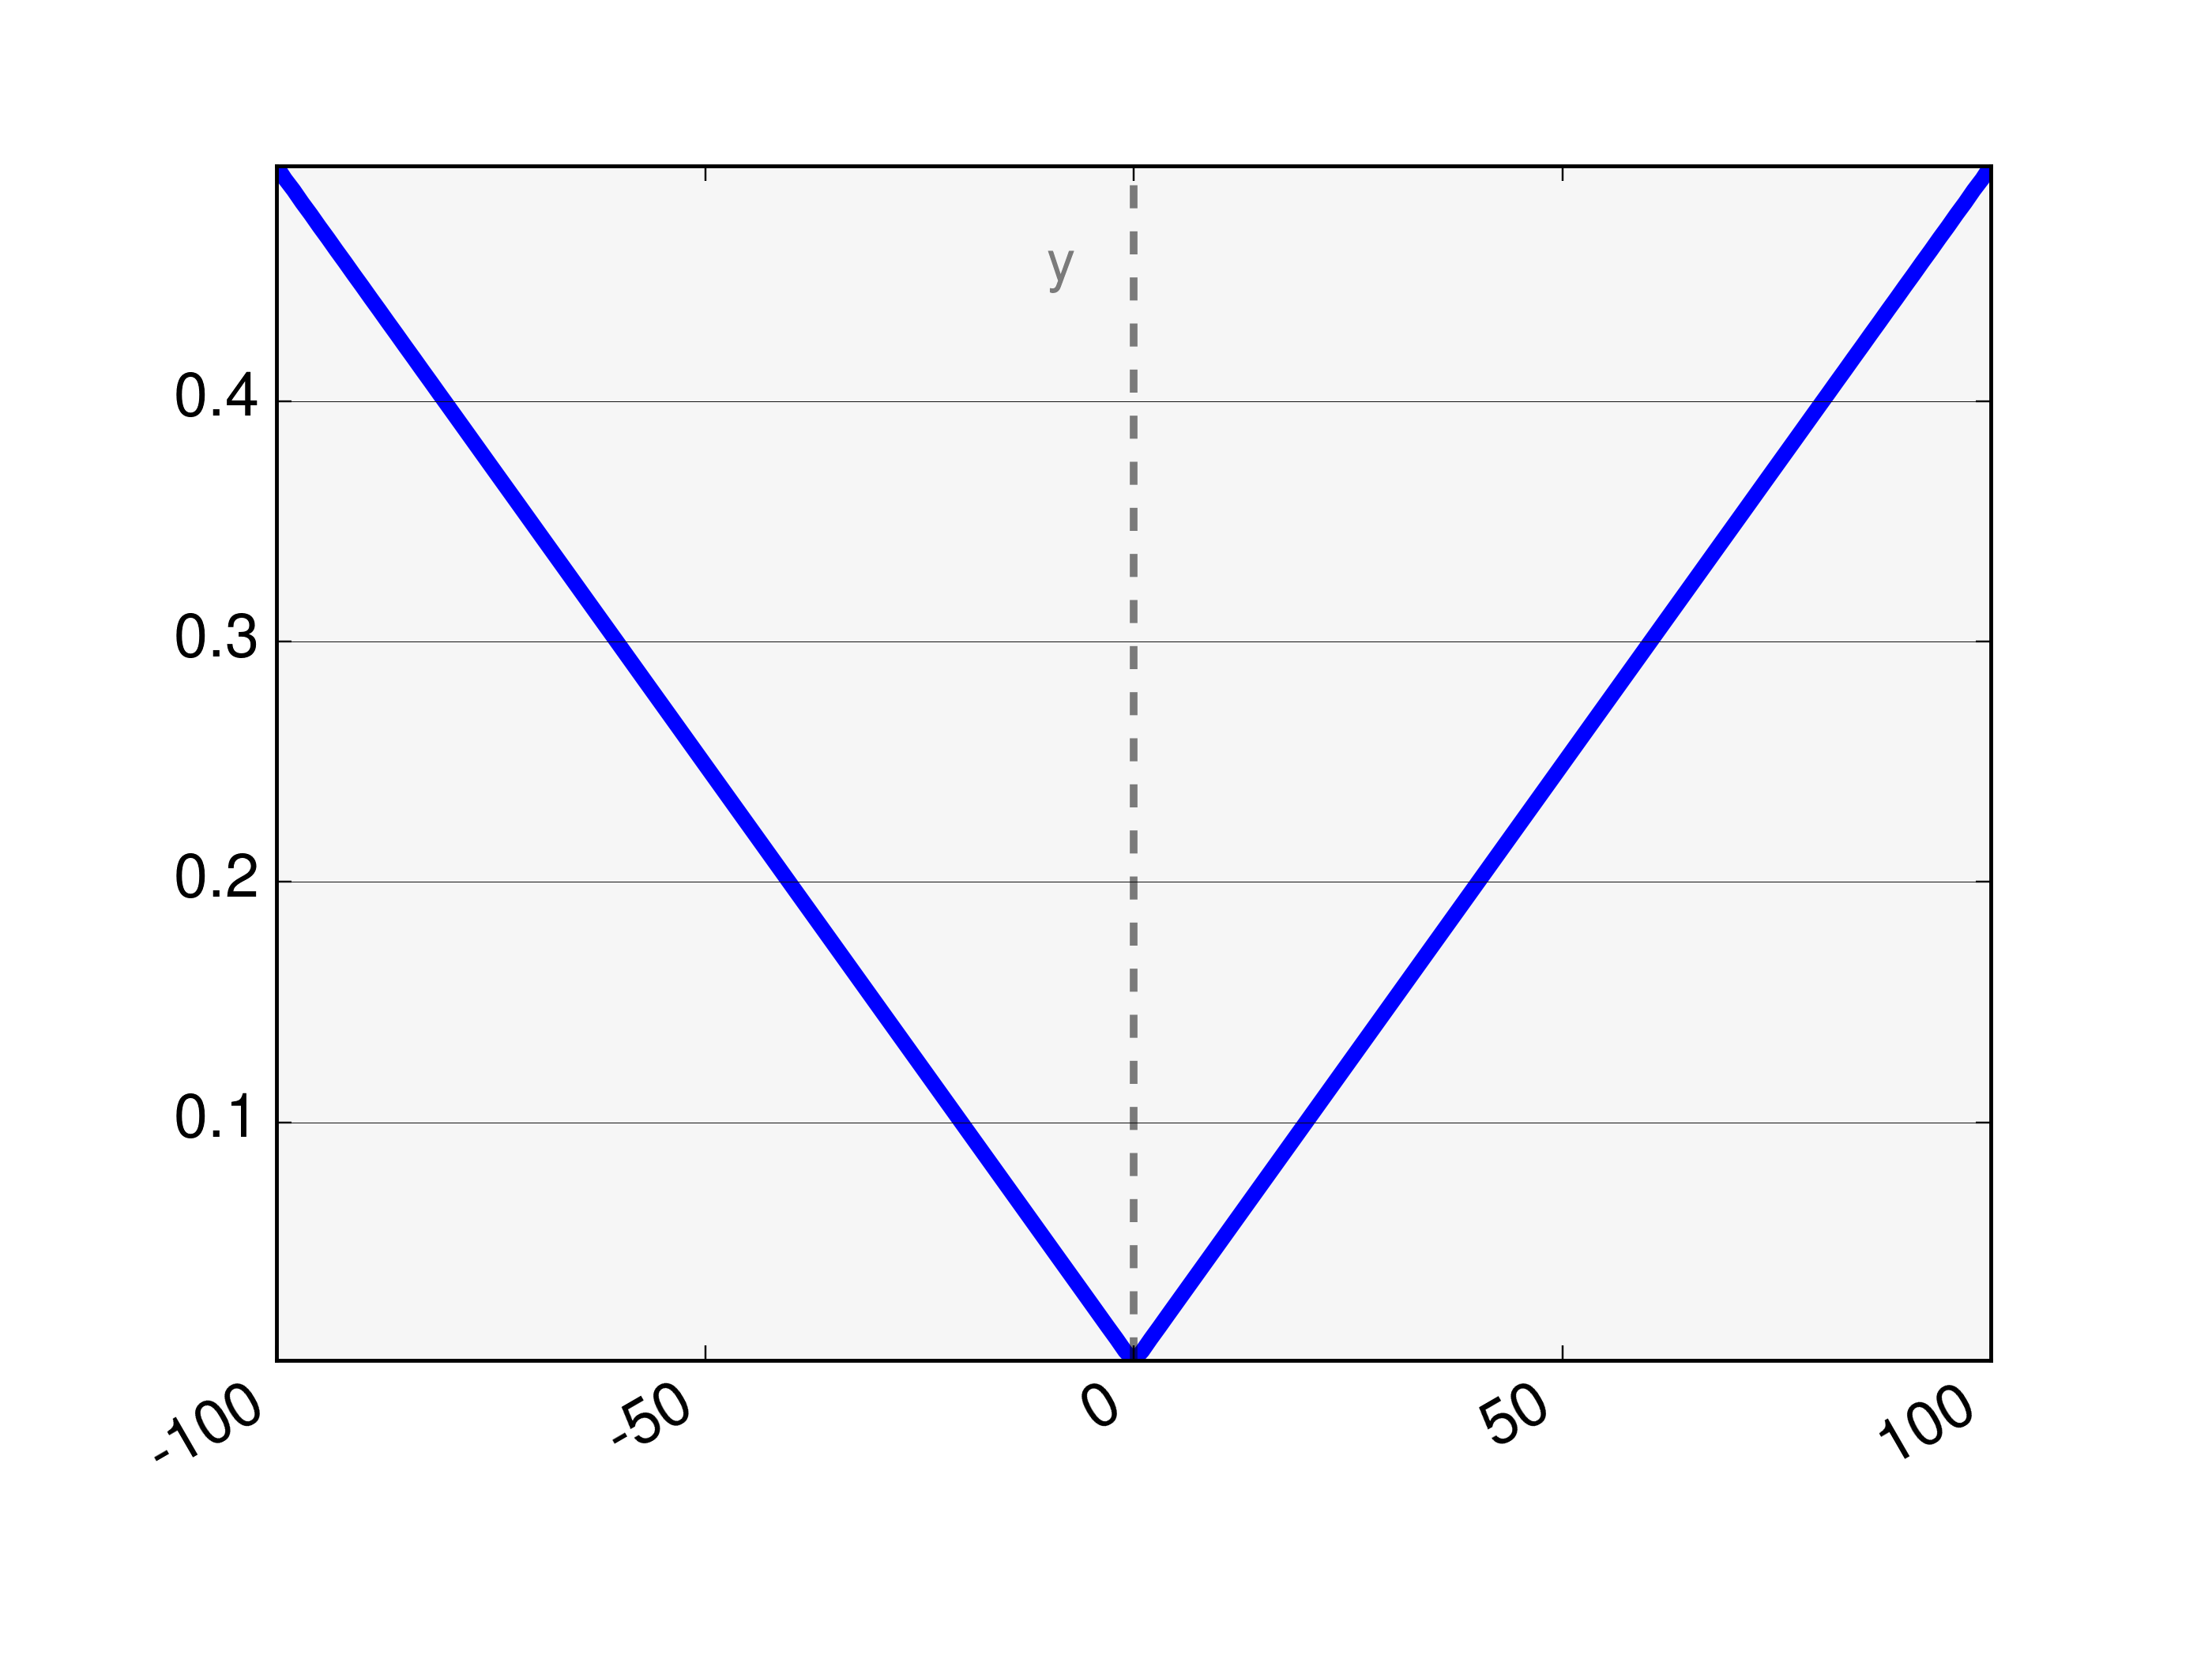
\includegraphics[width=8cm]{images/introduction_fbp_ramp_filter_fourier_space.png}\label{introduction:fbp:ramp-filter2}  }}%
   \caption[Ramp filter in real and Fourier domain.]{(a) Filter $h[j\tau]$ given in (\ref{introduction:analytical-reconstruction:filtering-step4}) used to filter projections in
             real domain. (b) DFT of $h[j\tau]$ used to filter projections in
             Fourier domain.}%
    \label{introduction:fbp:ramp-filter}%
\end{figure}
For the FST, the Fourier domain of the object is sampled in a polar fashion by the DFT
of the projections, thus, it is more sparsely sampled at higher frequencies.
\newline
As shown in (\ref{introduction:analytical-reconstruction:fbp1}) and (\ref{introduction:analytical-reconstruction:fbp2}),
projections can be either filtered in Fourier or real domain. The first solution can be efficiently implemented with FFT,
provided that the data are first zero-padded to avoid the \emph{wrap-around effect}. The convolution theorem is, indeed, 
applicable only to cyclic convolutions, i.e. the signals are assumed to be periodic.
Hence, if there is no periodicity and FFT is used to implement the convolution,
the tails of the signals wrap around, leading to undesirable artifacts.
\newline
Due to the high-pass nature of the ramp filter, the filtering step enhances the noise affecting the projections.
As a matter of fact, the ``pure'' ramp filter should be employed only with almost noiseless data. 
In general, the ramp filter is multiplied with a window, that ignores low frequencies and suppresses the highest frequencies to a certain extent.
Well-known examples of such windows are Shepp-Logan (abbr. ``sl''), Hanning (abbr. ``hn''),
Hamming (abbr. ``hm'') and 
Parzen (abbr. ``pz'') \cite{Lyra2011}, having the following expressions:
\begin{align*}
  & w_{\text{sl}}(f) = \frac{\displaystyle2\frac{f}{f_{c}}}{\displaystyle\pi \sin\left( \frac{\pi|f|}{2f_{c}} \right)} \nonumber\\[1em]
  &w_{\text{hn}}(f) = \begin{cases}\displaystyle
			  0.5 + 0.5 \cos\left(\frac{\pi f}{f_{c}}\right) & 0 \leq |f| \leq f_{c}\\
			  0 & \text{otherwise}
                       \end{cases}\nonumber\\[1em]
  & w_{\text{hm}}(f) = \begin{cases}\displaystyle
			  0.54 + 0.46 \cos\left(\frac{\pi f}{f_{c}}\right) & 0 \leq |f| \leq f_{c}\\
			  0 & \text{otherwise}
                       \end{cases} \nonumber\\[1em]
  &  w_{\text{pz}}(f) = \begin{cases}\displaystyle
			  |f| -6|f|\left(\frac{|f|}{f_{c}}\right)^{2} \left( 1 - \frac{|f|}{f_{c}} \right)  & \displaystyle 0 < |f| < \frac{f_{c}}{4}\\
			  \displaystyle 2|f|\left( 1 - \frac{|f|}{f_{c}} \right)^{2}  & \displaystyle \frac{f_{c}}{4} < |f| < \frac{f_{c}}{2}\\
			  0 & \displaystyle |f| \geq \frac{f_{c}}{2}
                       \end{cases}\nonumber\\                      
\end{align*}
where $f_{c}$ is the \emph{cutoff-frequency}, i.e. the high frequencies corresponding to $|f| > f_{c}$ are suppressed. 
Fig. \ref{introduction:fbp:filter-function-fourier-space}, where the four window functions are compared in the interval [0,1],
shows that high frequencies are suppressed the most by the Parzen window.
Since high frequencies correspond either to noise or highly varying signal features, the conclusion is that FBP reconstructions
with the ramp filter will have the best spatial resolution and the highest amount of noise, whereas those with the ramp filter combined to
the Parzen window will have the worst spatial resolution and the lowest amount of noise.
The filter function plays a crucial role in determining the reconstruction quality in terms of signal-to-noise ratio/spatial resolution trade-off.
For this reason, it is always mandatory,
especially in published works showing analytical tomographic reconstructions, to specify what kind of filter has been used for FBP.

\begin{figure}[!h]
    \centering
    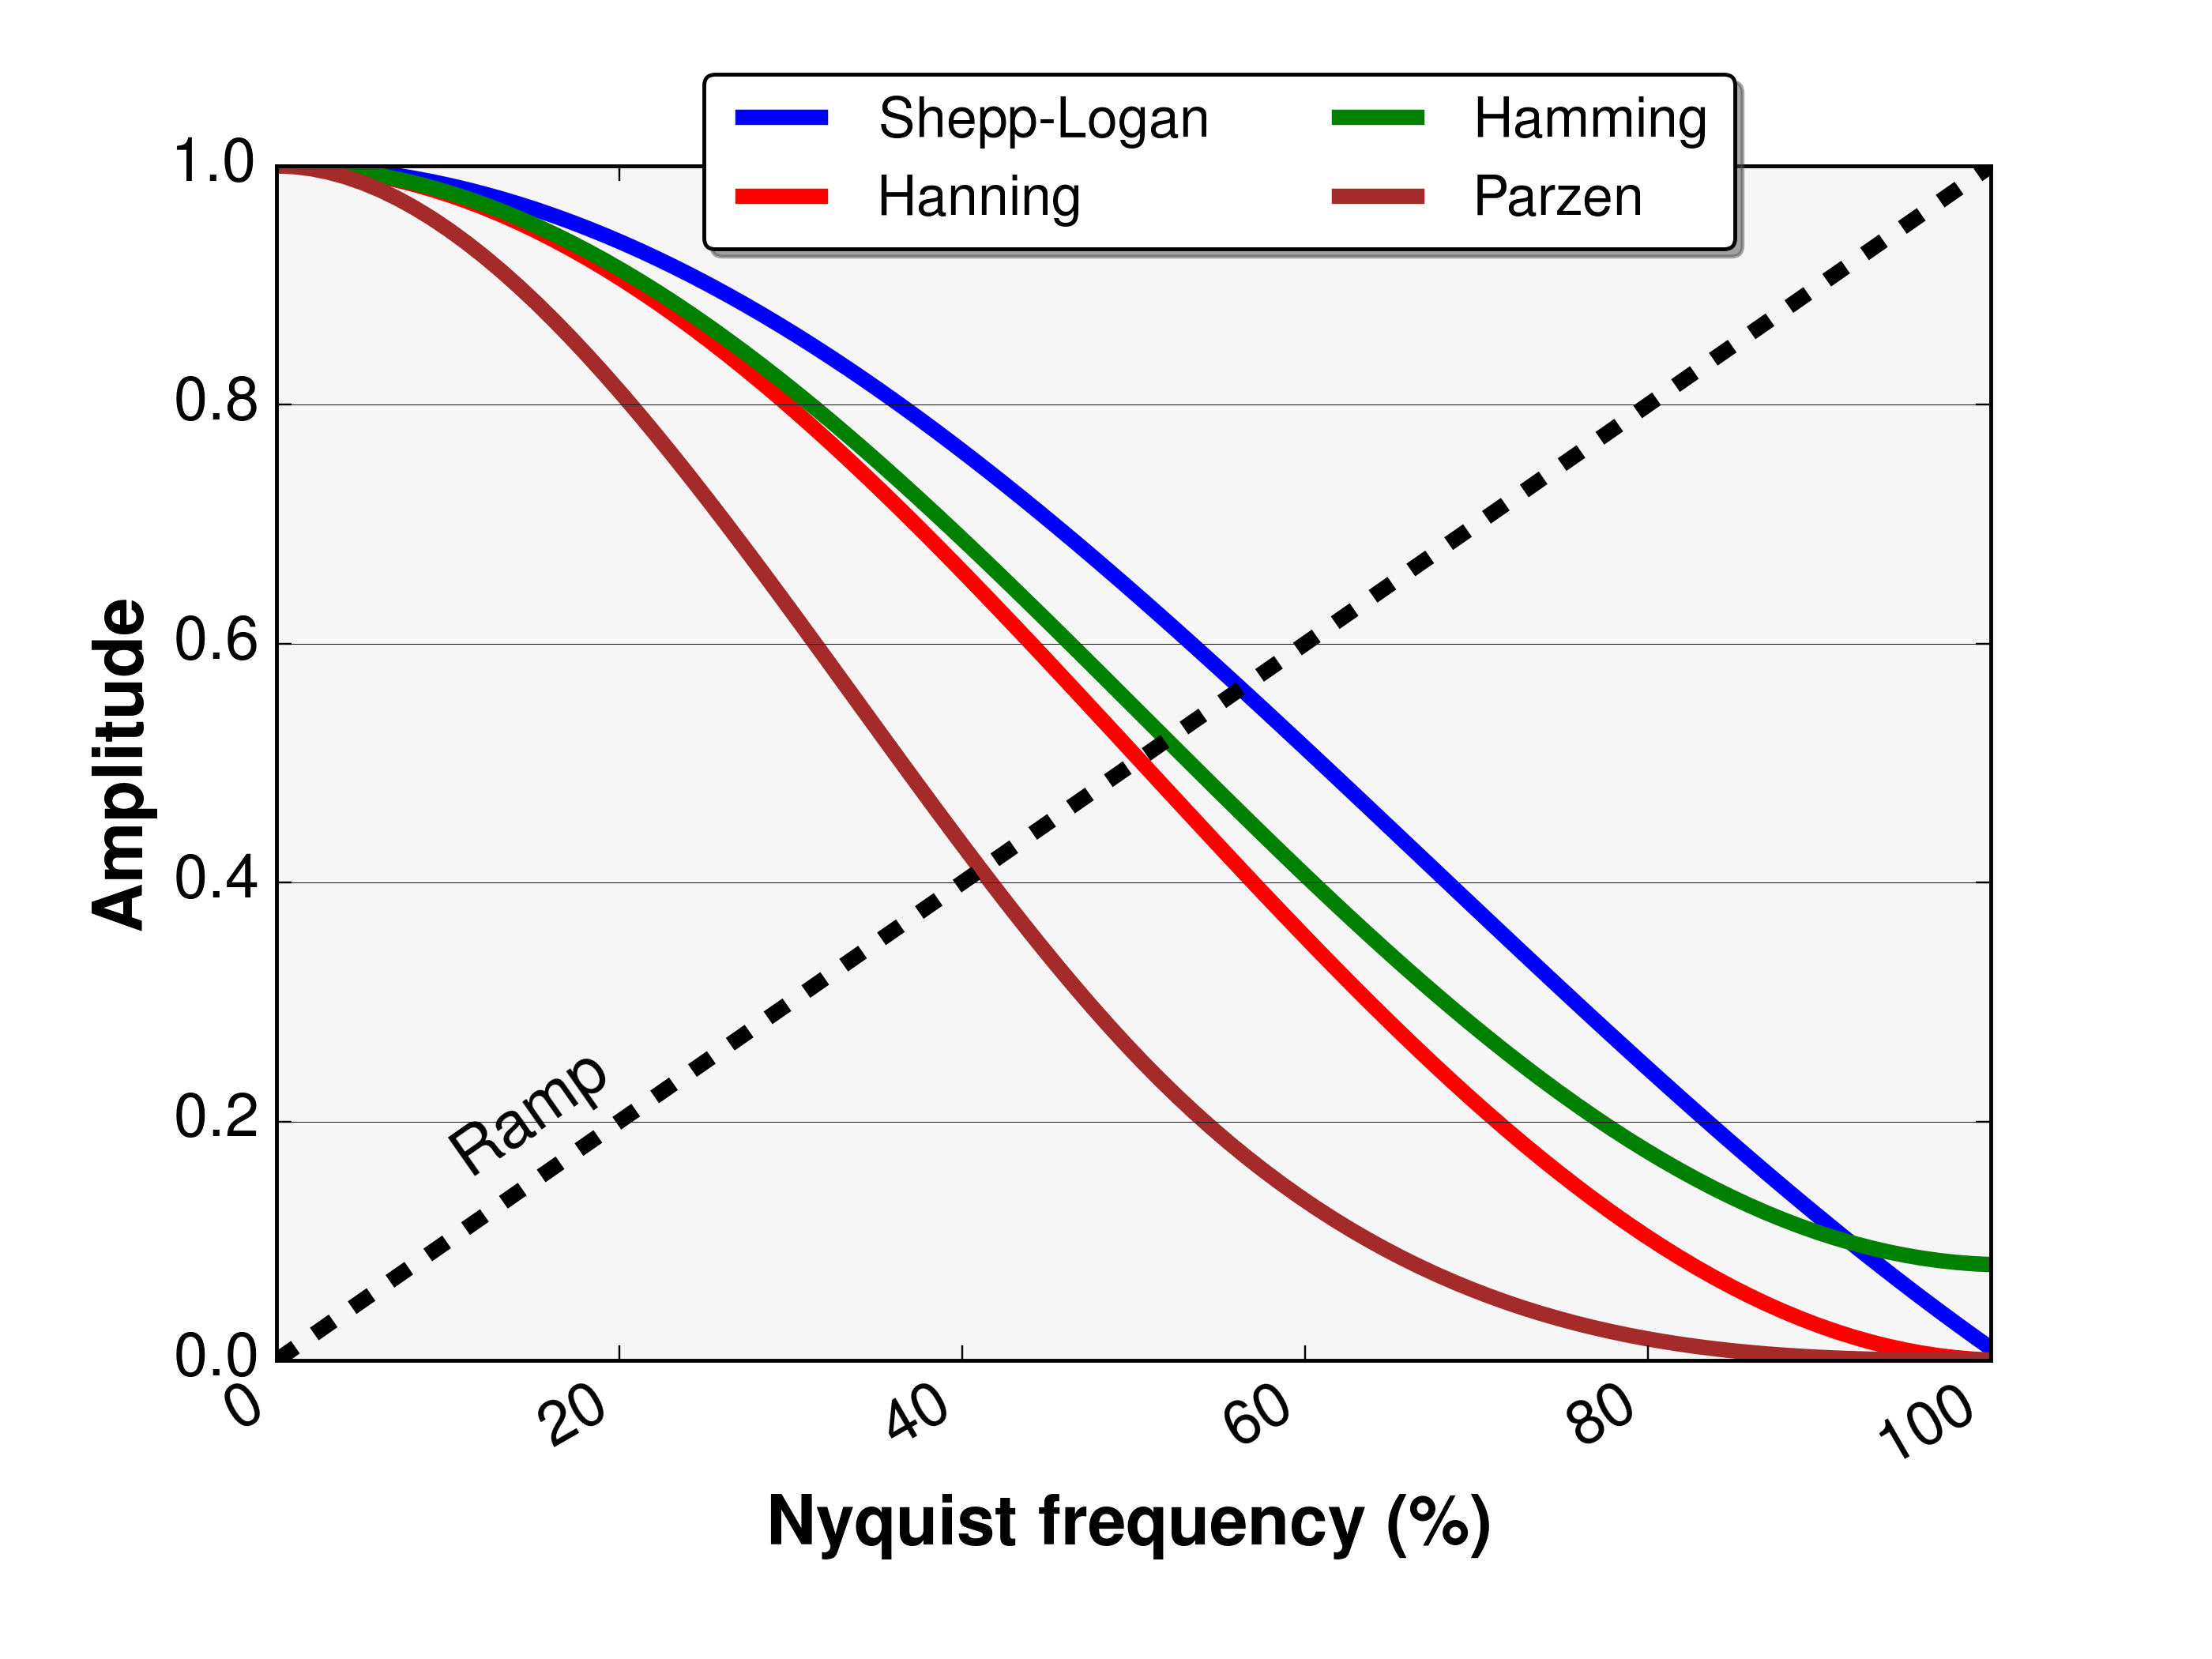
\includegraphics[width=11cm]{images/introduction_fbp_filter_function_fourier_space.png}   
   \caption[Low-pass windows that can be superimposed to the ramp filter.]{Shepp-Logan, Hanning, Hamming and Parzen windows at comparison.}
    \label{introduction:fbp:filter-function-fourier-space}
\end{figure}


\subsection{Implementation aspects of the discrete backprojection}
\label{introduction:analytical-reconstruction:discrete-backprojection}
The discrete backprojection formula (\ref{introduction:analytical-reconstruction:fbp4}) is schematically depicted in
Fig. \ref{introduction:fbp:backprojection}: consider a single data point belonging to a filtered projection,
$p^{(f)}[\theta,t]$; trace the X-ray line corresponding to that point, i.e. $r\,:\,x_{1}\cos\theta + x_{2}\sin\theta = t$;
assign the (scaled) data point to each image pixel traversed by $r$; do the same operation for the other data points;
repeat for all projections in $[0,\pi)$. All contributions from data points of different projections to the same image pixel
are summed up. The backprojection of all data points leads to an approximated version of the object $\mathbf{f}$.
\newline
Backprojection $\Backproject$ represents the \emph{adjoint operator} of the Radon transform $\Radon$,
i.e. $\Backproject = \Radon^{*}$. 
Given a generic linear operator $\Genop\::\: U \Longrightarrow V$, with $U, V$ being vector spaces,
the adjoint operator, $\Genop^{*}\::\: V \Longrightarrow U$, satisfies:
\begin{equation}
	\Big\langle  y\,,\, \Genop(x) \Big\rangle = \Big\langle  \Genop^{*}(y)\,,\, x \Big\rangle \hspace{0.8cm} \forall\,x \in U 
	\hspace{0.5cm} \forall y \in V \hspace{0.3cm}.
\end{equation}
From a computational point of view, the implementation of $\Genop^{*}$ consists
of the same (all linear) operations involved by $\Genop$, but in reverse order and with input/output arrays
exchanged (if $\Genop$ is complex, then, each adjoint calculation undergoes additional complex conjugation).
This means that every implementation scheme described in
\ref{introduction:radon-transform:real-space-implementations} can be used to build a corresponding backprojector. 
The complexity of all these algorithms is, at least, $\Complexity\left(N^{3}\right)$ 
\cite{Toft1996,Herman2009,Joseph1982,Deman2004,Lewitt1990,Horbelt2002}.
The computational hurdle of the backprojection operation can be greatly reduced through parallelized
implementations on Graphics Processing Units (GPUs). Two well-known examples of Open Source softwares
offering very fast GPU-based tomographic projectors have been published in \cite{Pedemonte2010,Palenstijn2011}.
\newline
An algorithm characterized by much lower complexity is the \emph{hierarchical backprojector} \cite{Basu2000}.
The idea is to split the reconstruction of an image $f^{(N)} \in \mathbb{R}^{N\times N}$ from a sinogram consisting,
for example, of $N$ views $\times$ $N$ pixels
into the reconstruction of 4 images with half number of pixels, namely, $f^{(N/2)} \in \mathbb{R}^{N/2\times N/2}$. 
A fairly accurate reconstruction of each $f^{(N/2)}$ requires only $N/2$ views, since the pixels are halved in both dimensions.
Backprojection for the 4 images $f^{(N/2)}$ requires approximately $4 \cdot (N/2)^{3} = N^{3}/2$ floating operations.
The recursive usage of this strategy of halving the image grid and the sinogram leads to an algorithm with complexity 
$\Complexity\left(N^{2}\log_{2}N\right)$ \cite{Basu2000}, making the hierarchical backprojector much faster than any of the 
previously mentioned FBP implementations. 

\begin{figure}[!t]
    \centering
    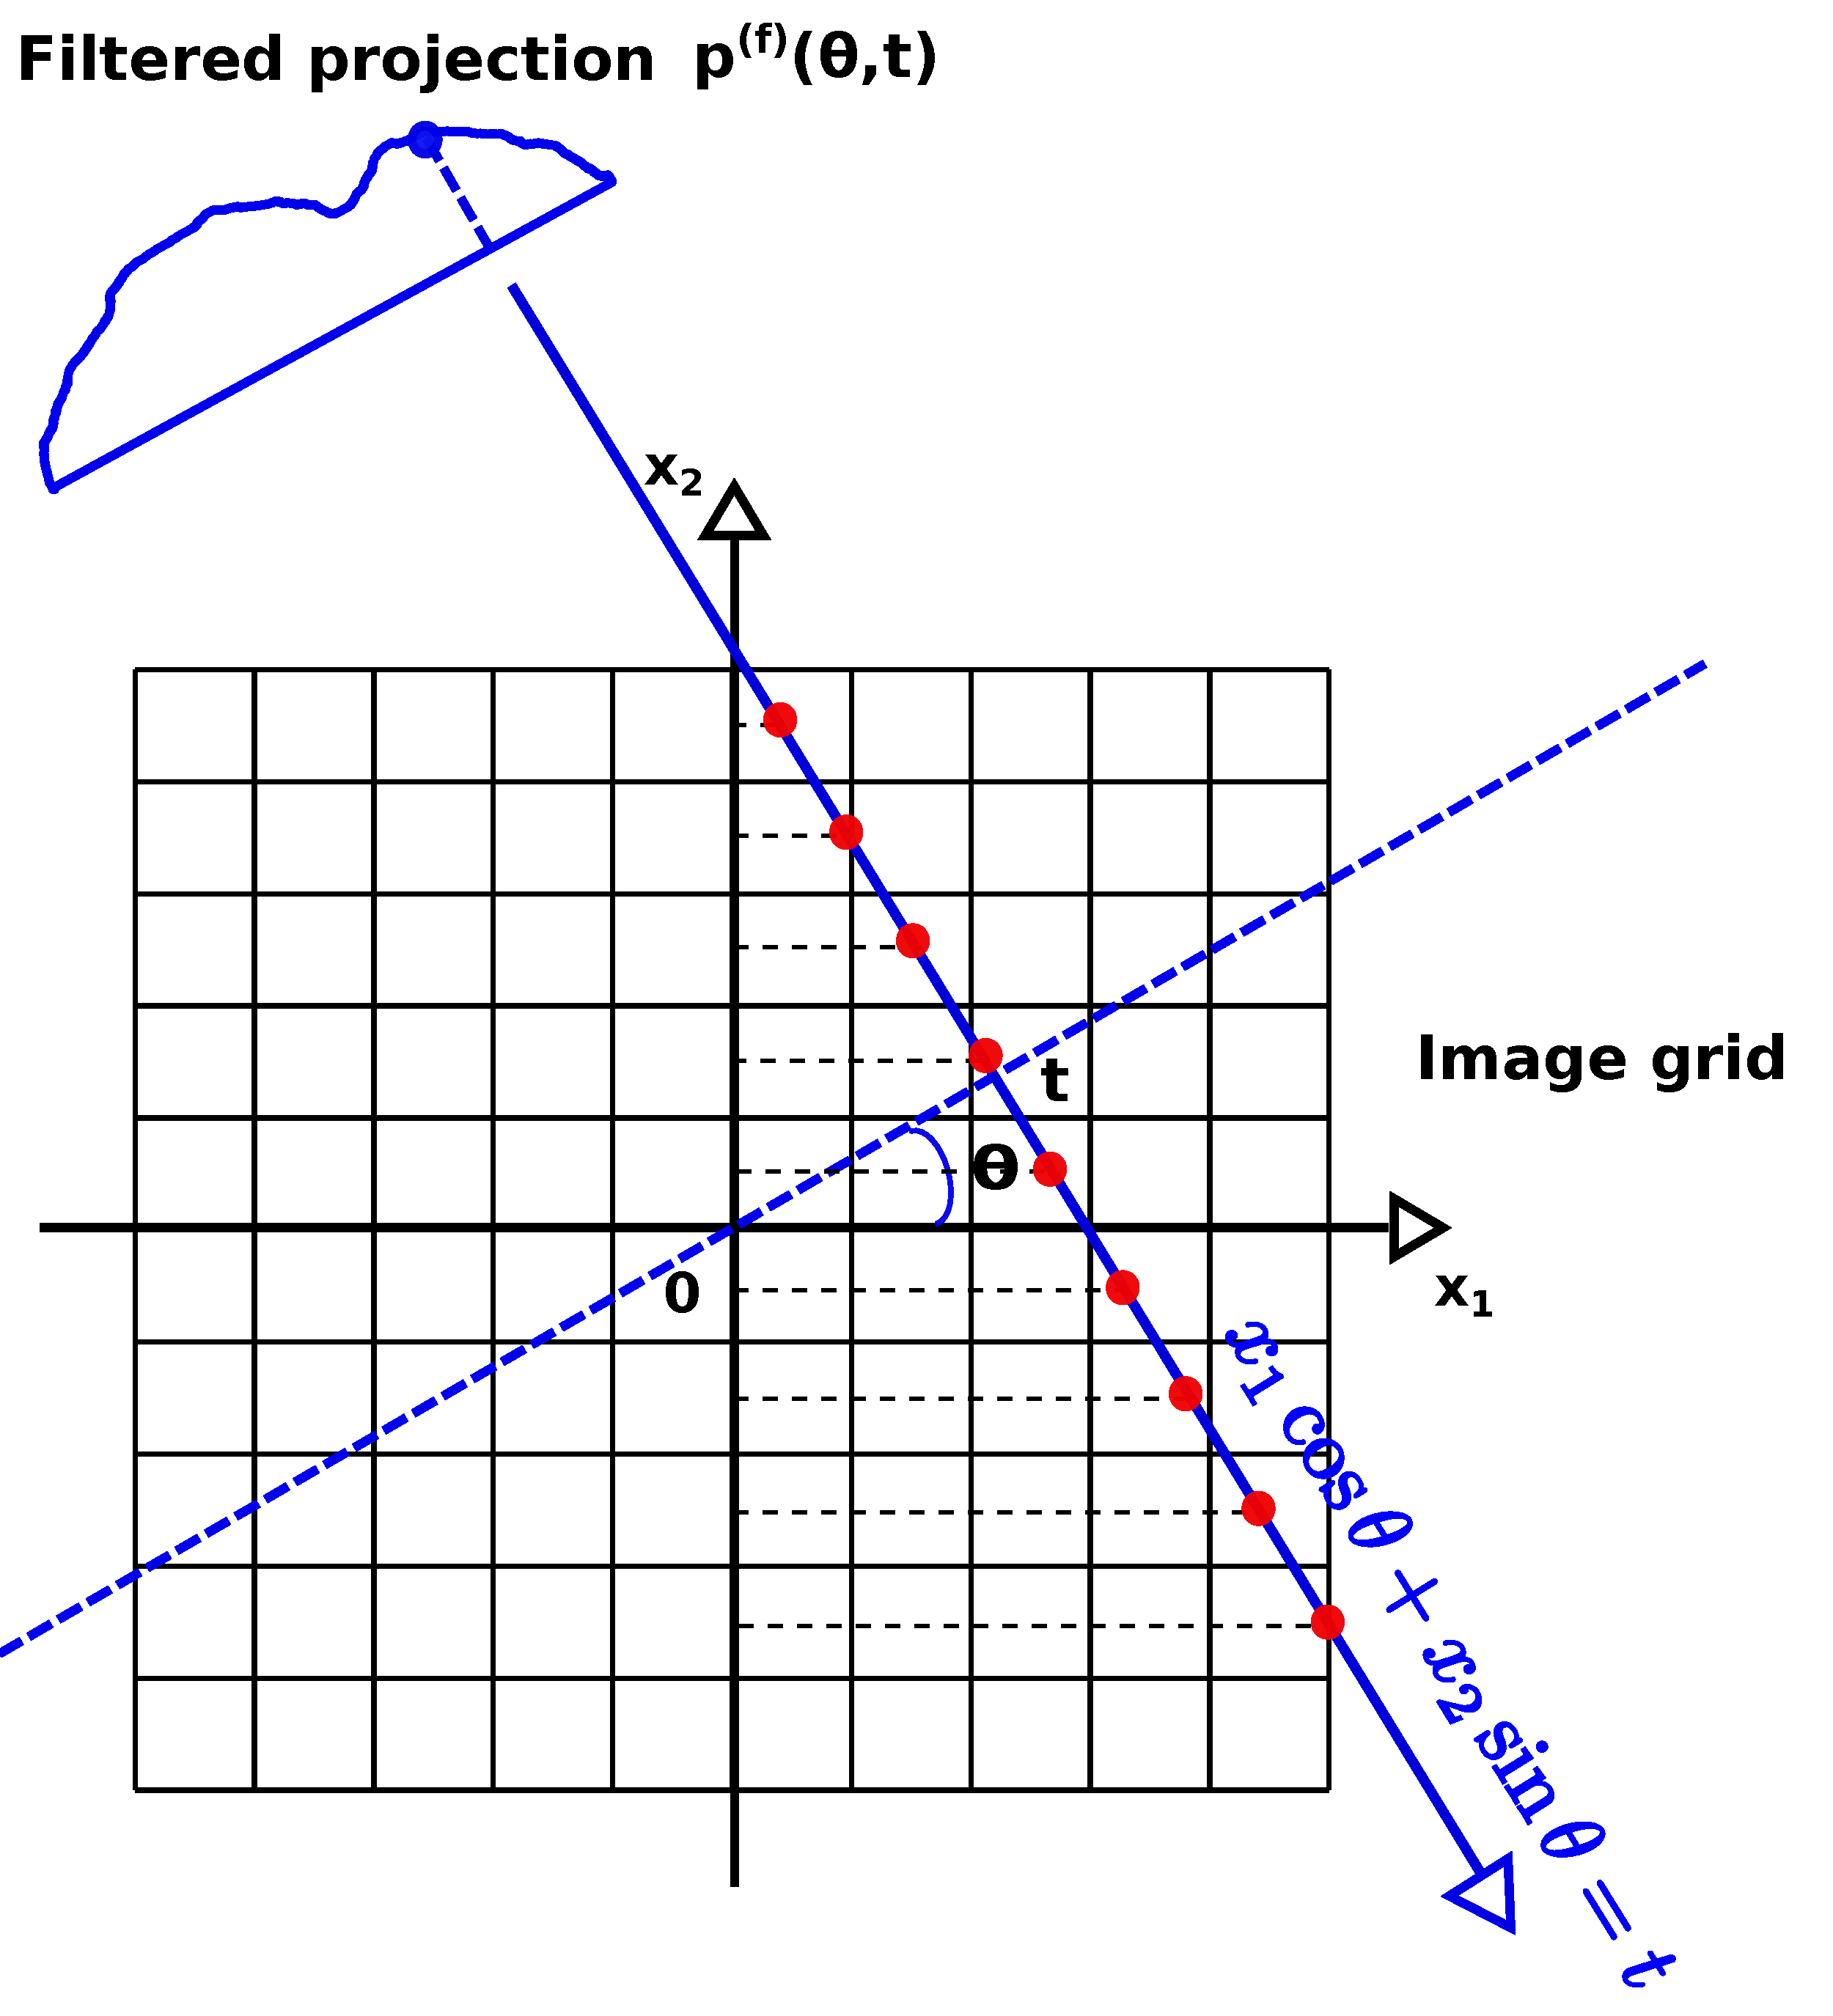
\includegraphics[width=8cm]{images/introduction_fbp_backprojection.pdf}   
   \caption[Sketch of the backprojection operation.]{Sketch of the backprojection operation.}
    \label{introduction:fbp:backprojection} 
\end{figure}



\section{Iterative reconstruction}
\subsection{Underconstrained datasets}
\label{introduction:underconstrained-datasets}
FBP has represented the standard CT reconstruction algorithm for decades, since its introduction.
This method is easy to understand, works fast with a parallel implementation and provides high-quality
reconstructions,
when the sinogram is ``properly'' sampled.
\newline
Practical rules of thumb discussed in \cite{Kak2001} suggest that the reconstruction of a $N\times N$ grid
requires $M \approx N \pi / 2$ projections homogeneously acquired in $[0,\pi)$, each sampled with $K \approx N$ data points.
When $M \approx N \pi / 2$ and $K \ll N$, the reconstruction is affected by thick streak artifacts due to the aliasing of single projections.
Thin streaks appear in case $M \ll N \pi / 2$ and $K \approx N$, giving rise to a characteristic star-shaped artifact \cite{Kak2001}.
In both scenarios, a sinogram in parallel beam geometry is regarded as \emph{undersampled} for FBP. 
\newline
Two sources of noise usually affect projection data: additive noise due to roundoff errors/electrical noise and shot noise, 
which is signal-dependent and follows a Poissonian statistics. Assuming the additive noise a stationary zero-mean random process
uncorrelated for different projections, it is possible to show that \cite{Kak2001}:
\begin{equation}
  \sigma_{r}^{2} = \sigma_{p}^{2}\:\pi\int\limits_{-\infty}^{+\infty} d\omega \: |\omega|^{2} \: |w(\omega)|^{2}
  \label{introduction:analytical-reconstruction:underconstrained-datasets1}
\end{equation}
where $\sigma_{r}$ is the standard deviation (std) of the FBP reconstruction, $\sigma_{p}$ is the std of the projection data
and $w(\omega)$ is the additional window function for the filtering step. 
Relation (\ref{introduction:analytical-reconstruction:underconstrained-datasets1}) shows that the smaller the area under 
$|\omega|^{2} \: |w(\omega)|^{2}$, the smaller the error affecting the final reconstruction, but the bigger the distortions
due to edge-blurring, as already stated in \ref{intruduction:analytical-reconstruction:filtering-step}. An expression
similar to (\ref{introduction:analytical-reconstruction:underconstrained-datasets1}) can be derived for the case of shot noise
\cite{Kak2001}.
\newline
Although the previous arguments are helpful in understanding the FBP performance under data insufficiency or noise,
the reconstruction algorithm needs always to be tested on experimental data acquired with the tomographic setup under study.
Effects like the non-zero size of the detector aperture function 
or some kind of structured noise characterizing the data can highly deviate the performance
of FBP (and any other reconstruction algorithm) from what theoretically expected. For example, a finite detector aperture function
acts roughly as a low-pass filter, that can suppress the potential aliasing of the projection data \cite{Kak2001}.
\newline
In this work, the term \emph{underconstrained} is used to generally identify tomographic datasets, for which
analytical algorithms like FBP are unable to provide high quality reconstructions. 
In the experimental practice, underconstrained datasets result from
low-dose fast scans or from tomographic setups, where projections cannot be acquired homogeneously in $[0,\pi)$.
The study conducted in this thesis focuses on the first case. Low-dose scans enable in-vivo studies that are
particularly relevant in biomedical research; fast scans allow tomography of quickly varying specimens of any kind.
To decrease total dose and scan time for a given CT setup, two possibilities are available:
acquiring a little number of projections, which leads to undersampled sinograms ($M \ll N \pi / 2$)\footnote{The case
$K \ll N$ is of no interest for SRXTM, due to the high-resolution detectors employed for these kind of tomographic scans.}; 
decreasing the exposure time per projection, that yields very noisy data.
Another current challenge in SRXTM is the reconstruction of \emph{interior tomography} data, arising when the irradiated 
object does not fit inside the CT field-of-view, leading to the acquisition of truncated projections.
Undersampled, noisy and truncated datasets (or a combination of these issues), whose reconstruction cannot be ``successfully''
tackled by means of FBP, are all here referred as underconstrained.


\subsection{Iterative methods}
\label{introduction:iterative-reconstruction}
The following paragraph does not want to be an extensive review of iterative methods for tomographic reconstruction. 
Some key aspects and the various ``families'' of iterative algorithms are here listed.
\newline
Iterative algorithms are non-linear methods designed to provide better reconstruction accuracy than FBP
when dealing with underconstrained datasets. Reconstructions are calculated through minimization of a cost function embedding 
a fidelity term, that steers the solution to fit the input data, and a regularization term, that pushes the solution to fulfill the 
expectations or a-priori knowledge of the object under study. Customary components are: a forward and a backprojection operator,
an iterative solver, a regularization scheme, constraints, a stopping criterion and parameters (supervised or unsupervised)
weighting the influence of each component. 
Iterative algorithms require more computations than FBP and the computational bottleneck usually lies in the few calls per iteration of 
the forward and backprojector. 3D compressed sensing based regularizations can easily represent a computational bottleneck as well
(more on this aspect in \ref{admm:notes-on-regularization}).
\newline
Algebraic methods were the first iterative algorithms to have ever been introduced. They include the algebraic reconstruction
technique (ART) \cite{Herman1973}, the simultaneous iterative reconstruction algorithm (SIRT) \cite{Gilbert1972} and the 
simultaneous algebraic reconstruction technique (SART) \cite{Andersen1984}. Algebraic methods treat the tomographic problem as a system
of equations, iteratively solved by the Kaczmarz method \cite{Kaczmarz1937}.
\newline
Bayesian methods incorporate the statistical model (usually a Poissonian or a compound of Poissonians)
ruling the signal formation at the detector.
The maximum likelihood expectation maximization (MLEM) \cite{Shepp1982},  
the penalized weighted least square method (PWLS) \cite{Fessler1994,Erdogan1999,Elbakri2002} belong to this group of algorithms.
\newline
Modern techniques for convex optimization like the split Bregman method \cite{Goldstein2009}
and the alternate direction method of multipliers (ADMM) \cite{Boyd2010} have recently been applied to tomographic reconstruction
\cite{Wang2012,Ramani2012,Chun2014}. 
\newline
The projection-onto-convex-sets (POCS) method \cite{Gubin1967} is designed to find the intersection area of
closed convex sets and has been mainly used to address the interior tomography problem combined to differentiated backprojection
\cite{Defrise2006}.
\newline
Discrete tomography algorithms \cite{Herman1999} deal with the reconstruction of images whose domain is a discrete set.
Some studies focus on the reconstruction of binary images \cite{Schle2005,Batenburg2007}, others contemplate reconstruction problems
involving any small number of grey levels \cite{Alpers2006,Liao2005}. The discrete algebraic reconstruction technique (DART) \cite{Batenburg2011}
is a recent approach designed for discrete tomography, that combines both non-discrete and discrete update steps at each iteration.
\newline
Iterative methods incorporate regularization schemes to stabilize the inversion problem and to improve the reconstruction accuracy
by exploiting some kind of a-priori knowledge regarding the object under study.
Examples of ``classical'' regularization schemes are Tikhonov \cite{Tikhonov1977} and Huber \cite{Huber1964} penalties.
Regularization schemes based on compressive sensing \cite{Donoho2006} like total variation (TV) \cite{Rudin1992} are described in 
\ref{admm:notes-on-regularization}.
}
